% Clase del documento
\documentclass[12pt,twoside,titlepage]{report}

%%%%%%%%%%%%%%%%%%%%%%% Paquetes %%%%%%%%%%%%%%%%%%%%%%%

\usepackage[a4paper,bindingoffset=3mm,bottom=35mm]{geometry}

% Usad \usepackage[dvips]{graphicx} o \usepackage[pdftex]{graphicx} (no ambos)
%\usepackage[dvips]{graphicx} %%% para LaTeX. Las figuras deben estar en formato eps

\usepackage[colorlinks=true,pdftex]{hyperref}   %%% Opcional. Para incluir marcadores y enlaces en el pdf
\usepackage[pdftex]{graphicx}  %%% para pdflatex. Las figuras pueden estar en pdf, jpg, svg y otros formatos

\usepackage[spanish]{babel}

%\usepackage[latin1]{inputenc} % Usad en WinEdt/MikTex
\usepackage[utf8]{inputenc} % Usad en overleaf

\usepackage[T1]{fontenc} % necesario para «comillas latinas» y guiones en español

% Algunos paquetes útiles

\usepackage{amsmath,amssymb}
\usepackage{color}
\usepackage{afterpage}
\usepackage{paralist}
\usepackage{array}
\usepackage{enumerate}
\usepackage{enumitem}
\usepackage{float}
\usepackage{setspace}
\usepackage{listings}
\usepackage{algorithm}
\usepackage{algorithmic}
\usepackage{fancyhdr}
\usepackage{rotating}
\usepackage{multirow}
\usepackage{microtype}

% Otros paquetes

\usepackage{quotchap}

\usepackage{tikz}
\usetikzlibrary{arrows.meta, positioning, calc}

%%%%%%%%%%%%%%%%%%%%%%%%%%%%%%%%%%%%%%%%%%%%%%%%%%%%%%%%

%%%%%%%%%%%%%%%%%%%%%%% Definiciones básicas %%%%%%%%%%%%%%%%%%%%%%%

\newcommand{\nombreautor}{Cristina Lozano Bautista}
\newcommand{\nombretutor}{Aaron Sujar}
% Título propuesto — ajustar si se prefiere otro:
\newcommand{\titulotrabajo}{Sprout: Prototipo de videojuego narrativo con agentes basados en modelos de lenguaje}
\newcommand{\escuela}{Escuela Técnica Superior\\de Ingeniería Informática}
\newcommand{\escuelalargo}{Escuela Técnica Superior de Ingeniería Informática}
\newcommand{\universidad}{Universidad Rey Juan Carlos}
\newcommand{\fecha}{Junio de 2026}
\newcommand{\grado}{Grado en Diseño y Desarrollo de Videojuegos}
\newcommand{\curso}{Curso 2025-2026}
\newcommand{\logoUniversidad}{logoURJC.pdf} % logoURJC.eps


\newcommand{\revisar}[1]{\textcolor{red}{\underline{#1}}}


%%%%%%%%%%%%%%%%%%%%%%%%%%%%%%%%%%%%%%%%%%%%%%%%%%%%%%%%%%%%%%%%%%%%

%%%%%%%%%%%%%%%%%%%%%%%%% Otras definiciones %%%%%%%%%%%%%%%%%%%%%%%%%%

% Definiciones de colores (para hidelinks)
\definecolor{BlueLink}{rgb}{0.165,0.322,0.745}
\definecolor{PinkLink}{rgb}{0.8,0.22,0.5}
\definecolor{gray}{rgb}{0.6,0.6,0.6}

% Enlaces
\hypersetup{hidelinks,pageanchor=true,colorlinks,citecolor=PinkLink,urlcolor=black,linkcolor=BlueLink}

\newcommand\blankpage{%
    \newpage
    \null
    \thispagestyle{empty}%
    %\addtocounter{page}{-1}%
    \newpage}

% Texto referencias
\addto{\captionsspanish}{\renewcommand{\bibname}{Bibliografía}}

% Texto Índice de tablas
\addto\captionsspanish{
\def\tablename{Tabla}
\def\listtablename{\'{I}ndice de tablas}
}

\floatname{algorithm}{Algoritmo}

%\newenvironment{pseudocodigo}[1][htb]
%  {\renewcommand{\algorithmcfname}{Pseudocódig}% Update algorithm name
%   \begin{algorithm}[#1]%
%  }{\end{algorithm}}

%%%%%%%%%%%%%%%%%%%%%%%%%%%%%%%%%%%%%%%%%%%%%%%%%%%%%%%%%%%%%%%%%%%%

%%%%%%%%%%%%%%%%%%%%%%% Estilo de código %%%%%%%%%%%%%%%%%%%%%%%

\definecolor{bg}{rgb}{0.95,0.95,0.95}
\definecolor{mydeepteal}{rgb}{0.16,0.22,0.23}
\definecolor{myteal}{rgb}{0.31,0.44,0.46}
\definecolor{mymediumteal}{rgb}{0.41,0.58,0.60}

\DeclareFixedFont{\ttb}{T1}{txtt}{bx}{n}{12} % for bold
\DeclareFixedFont{\ttm}{T1}{txtt}{m}{n}{12}  % for normal

%\newcommand*{\FormatDigit}[1]{\textcolor{mydeepteal}{#1}}
\newcommand*{\FormatDigit}[1]{\textcolor{black}{#1}}

% Estilo por defecto de los listados (prompts y fragmentos de C#)
\lstset{
basicstyle=\ttfamily\small,
showstringspaces=false,
backgroundcolor=\color{bg},
rulecolor=\color{bg},
breaklines=true,
numbers=left,
numbersep=5pt,
numberstyle=\tiny,
tabsize=4,
xleftmargin=1em,
frame=single,
framesep=3pt,
upquote=true,
literate={á}{{\'a}}1 {é}{{\'e}}1 {í}{{\'i}}1 {ó}{{\'o}}1 {ú}{{\'u}}1 {ñ}{{\~n}}1 {Á}{{\'A}}1 {É}{{\'E}}1 {Í}{{\'I}}1 {Ó}{{\'O}}1 {Ú}{{\'U}}1 {Ñ}{{\~N}}1 {¿}{{?`}}1 {¡}{{!`}}1
}

% Python style for highlighting
\newcommand\mypythonstyle{\lstset{
language=Python,
basicstyle=\ttfamily\small,
otherkeywords={self},
keywordstyle=\bfseries\ttfamily\color{myteal},
commentstyle=\itshape\color{myteal},
stringstyle=\color{mydeepteal},
emph={MyClass,__init__},
emphstyle=\ttb\color{mydeepteal},
showstringspaces=false,
backgroundcolor=\color{bg},
rulecolor = \color{bg},
breaklines=true,
numbers=left,
numbersep=5pt,
numberstyle=\tiny,
tabsize=4,
xleftmargin=1em,
frame = single,
framesep = 3pt,
framextopmargin=0pt,
framexbottommargin=0pt,
framexleftmargin=0pt,
framexrightmargin=0pt,
fontadjust=true,
basewidth=0.55em,
upquote=true,
}}

% Python environment
\lstnewenvironment{mypython}[1][]
{
\mypythonstyle
\lstset{#1}
}
{}

\newcommand\mypythoninline[1]{{\lstinline!#1!}}

%%%%%%%%%%%%%%%%%%%%%%%%%%%%%%%%%%%%%%%%%%%%%%%%%%%%%%%%%%%%%%%%%%%%%%%%%%%%%%

%%%%%%%%%%%%%%%%%%%%%%%%%%%% Comandos definidos por el autor

\newcommand{\transpuesta}{\mbox{\tiny $\mathsf{T}$}}

%%%%%%%%%%%%%%%%%%%%%%%%%%%%%%%%%%%%%%%%%%%%%%%%%%%%%%%%%%%%%%%%%%%%%%%
%                           Inicio del documento
%%%%%%%%%%%%%%%%%%%%%%%%%%%%%%%%%%%%%%%%%%%%%%%%%%%%%%%%%%%%%%%%%%%%%%%

\begin{document}

\pagestyle{plain}

%%%%%%%%%%%%%%%%%%%%%%%%%%%%%%%%%%%% Portada %%%%%%%%%%%%%%%%%%%%%%%%%%%%%%%%%%

% Universidad, Facultad
\begin{titlepage}
\selectlanguage{spanish}

% logo
\begin{center}
    \includegraphics[scale=0.7]{\logoUniversidad}
\end{center}

\bigskip

\begin{center}
\begin{LARGE}
\escuela \\
\end{LARGE}
\end{center}

\bigskip
\bigskip

% Grado
\begin{center}
\begin{large}
\textbf{\grado}\\
\end{large}
\end{center}

% Curso
\begin{center}
\begin{large}
\textbf{\curso}\\
\end{large}
\end{center}

\bigskip

\textbf{\begin{center}
\begin{large}
\textbf{Trabajo Fin de Grado}
\end{large}
\end{center}}

\bigskip
\bigskip
\bigskip

% Nombre del TFG
\begin{center}
\textbf{\begin{large}
\MakeUppercase{\titulotrabajo}\\
\end{large}}
\end{center}

% Nombre del autor
\vspace{\fill}
\begin{center}
\textbf{Autor: \nombreautor}\\ \smallskip
% Tutor
\textbf{Tutor: \nombretutor}\\
% Añadir segundo tutor si hubiera

\bigskip

% Fecha
%\textbf{\fecha}\\
\end{center}
\end{titlepage}

\hypersetup{pageanchor=true}

\normalsize
\afterpage{\blankpage} % Se deben añadir página en blanco para que lo capítulos de la memoria o estas secciones introductorias empiecen en páginas impares

%%%%%%%%%%%%%%%%%%%%%%%%%%%%%%%%%%%%%%%%%%%%%%%%%%%%%%%%%%%%%%%%%%%%%%%%%%%%%%%

% Estilo de párrafo de los capítulos
\setlength{\parskip}{0.75em}
\renewcommand{\baselinestretch}{1.25}
% Interlineado simple
\spacing{1}

\pagenumbering{Roman}
\setcounter{page}{2}

%%%%%%%%%%%%%%%%%%%%%%%%% Agradecimientos o dedicatoria %%%%%%%%%%%%%%%%%%%%%%%%%%%

\chapter*{Agradecimientos}

Breves agradecimientos o dedicatoria.

\afterpage{\blankpage}

%%%%%%%%%%%%%%%%%%%%%%%%%%%%%%%%%%%%%%%%%%%%%%%%%%%%%%%%%%%%%%%%%%%%%%%%%%%%%%%%%%%

%%%%%%%%%%%%%%%%%%%%%%%%%%%%%%%%%%%% Resumen %%%%%%%%%%%%%%%%%%%%%%%%%%%%%%%%%%%%%%

\chapter*{Resumen}

La evaluación del pensamiento divergente mediante instrumentos como los Tests de Torrance (TTCT) suele realizarse en contextos de examen que el propio carácter evaluativo puede condicionar. Este Trabajo Fin de Grado presenta \textit{Sprout}, un prototipo de videojuego narrativo en el que la jugadora regenta una floristería en un pequeño pueblo y conversa con cuatro personajes gobernados por un modelo de lenguaje a gran escala. Mientras conversa con naturalidad, el juego estima de forma implícita cuatro dimensiones del pensamiento divergente inspiradas en las subpruebas verbales del TTCT ---fluidez, flexibilidad, originalidad y elaboración---, sin que la jugadora perciba contexto evaluativo alguno.

El sistema se sustenta sobre una arquitectura en capas con un dominio de lógica pura, independiente del motor, y sobre una herramienta propia: un editor visual de grafos de diálogo construido sobre la API GraphView del editor de Unity, que constituye el eje técnico del proyecto. El modelo de lenguaje desempeña un triple papel ---generación de diálogo en personaje, clasificación de la intención del jugador y evaluación de las ideas---, y las medidas resultantes se materializan en mecánicas jugables (flores emocionales, cotilleo nocturno y finales múltiples) en lugar de mostrarse como puntuaciones numéricas.

El alcance del trabajo es el de un prototipo funcional: se documenta el comportamiento del sistema, pero su validación psicométrica queda explícitamente fuera de alcance y se plantea como principal línea de trabajo futuro. La memoria detalla el diseño, la implementación técnica y el protocolo de evaluación de usabilidad y experiencia diseñado para el prototipo, cuya ejecución con participantes se plantea igualmente como trabajo futuro.

\mbox{} \bigskip

\noindent \textbf{Palabras clave}:
\begin{compactitem}
    \item Pensamiento divergente
    \item Tests de Torrance (TTCT)
    \item IA conversacional
    \item Modelos de lenguaje a gran escala (LLM)
    \item Videojuego narrativo
    \item Evaluación implícita
\end{compactitem}

\afterpage{\blankpage}

%%%%%%%%%%%%%%%%%%%%%%%%%%%%%%%%%%%%%%%%%%%%%%%%%%%%%%%%%%%%%%%%%%%%%%%%%%%%%%%%%%%

%%%%%%%%%%%%%%%%%%%%%%%%%%%%%%%%%%%% Índices %%%%%%%%%%%%%%%%%%%%%%%%%%%%%%%%%%%%

% Estilo de párrafo de los Índices
\setlength{\parskip}{1pt}
\renewcommand{\baselinestretch}{1}
\renewcommand{\contentsname}{Índice de contenidos}

% Índice de contenidos
\tableofcontents
\afterpage{\blankpage}

% Índice de tablas (OPCIONAL)
\listoftables
\afterpage{\blankpage}
\addcontentsline{toc}{chapter}{\noindent \listtablename}

% Índice de figuras (OPCIONAL)
\listoffigures
\afterpage{\blankpage}
\addcontentsline{toc}{chapter}{\listfigurename}

% Índice de códigos/algoritmos (OPCIONAL)
\renewcommand\lstlistlistingname{Códigos}
\renewcommand\lstlistingname{Código}
\renewcommand\lstlistlistingname{Índice de códigos}

\lstlistoflistings
\afterpage{\blankpage}
\addcontentsline{toc}{chapter}{\lstlistlistingname}

%%%%%%%%%%%%%%%%%%%%%%%%%%%%%%%%%%%%%%%%%%%%%%%%%%%%%%%%%%%%%%%%%%%%%%%%%%%%%%%%%%%

%%%%%%%%%%%%%%%%%%%%%%% Cabeceras y pies de página (Opcional) %%%%%%%%%%%%%%%%%%%%%%%

%\setlength{\headheight}{15.2pt}
\pagestyle{fancy}

\renewcommand{\chaptermark}[1]{\markboth{Capítulo \thechapter.\ #1}{}}

\pagestyle{fancy}
\fancyhf{}
\fancyhead[LO]{\leftmark}
\fancyhead[RO]{}
\fancyhead[RE]{\nouppercase\rightmark}
\fancyhead[LE]{}
\fancyfoot[C]{\thepage}

%%%%%%%%%%%%%%%%%%%%%%%%%%%%%%%%%%%%%%%%%%%%%%%%%%%%%%%%%%%%%%%%%%%%%%%%%%%%%%%%%%%%

%%%%%%%%%%%%%%%%%%%%%%%%%%%%%% Capítulos de la memoria %%%%%%%%%%%%%%%%%%%%%%%%%%%%%

% Capítulo 1
\chapter{Introducción}

%%%%%%%%%%%%%%%%%%%%%%%%%%%%%%%%%%%%%%%%%%%%%%%%%%%%%%%%%%%%%%%%%%%%%%%%%%

% Estilo resto de páginas
\pagestyle{fancy}

% Estilo de párrafo de los capítulos
\setlength{\parskip}{0.75em}
\renewcommand{\baselinestretch}{1.25}
% Interlineado simple
\spacing{1}
% Numeración contenido
\pagenumbering{arabic}
\setcounter{page}{1}

%%%%%%%%%%%%%%%%%%%%%%%%%%%%%%%%%%%%%%%%%%%%%%%%%%%%%%%%%%%%%%%%%%%%%%%%%%

\section{Motivación}

Este Trabajo Fin de Grado nace de una pregunta que rara vez se hace en la intersección entre videojuegos e investigación psicológica: ¿puede un videojuego evaluar habilidades cognitivas sin que el jugador perciba que está siendo evaluado? La hipótesis de la que parte Sprout es que sí, y que el medio idóneo para hacerlo es una experiencia narrativa conversacional con personajes gobernados por inteligencia artificial. El motivo es estructural: el propio Torrance, creador del instrumento más utilizado para medir la creatividad, advertía ya en 1972 que la palabra ``test'' debía evitarse delante del participante para no inhibir las respuestas creativas. Sprout lleva ese principio hasta su consecuencia última: la evaluación no se disfraza de juego, es un juego.

Para responder a esa pregunta, el proyecto se sitúa deliberadamente en el cruce de tres campos que rara vez coinciden en un mismo trabajo. La psicología de la creatividad aporta el constructo a medir ---el pensamiento divergente--- y un instrumento de referencia con casi sesenta años de vigencia, cuyas prescripciones de aplicación resultan sorprendentemente compatibles con el diseño de juegos. El diseño de videojuegos aporta el medio: un espacio donde el participante actúa motivado por la propia experiencia, sin la presión de rendimiento que caracteriza a la situación de examen. Y los modelos de lenguaje a gran escala aportan la pieza que hasta hace muy poco faltaba para unir los dos anteriores: la capacidad de sostener una conversación abierta en lenguaje natural y, al mismo tiempo, de analizar semánticamente lo que la jugadora escribe.

La elección de la creatividad como objeto de medida no es casual. Nace de una inquietud personal de la autora ante el auge de la inteligencia artificial y su posible efecto sobre la creatividad infantil: los juegos simbólicos de toda la vida —jugar a las maestras, a los leones, a las muñecas— compiten hoy con el móvil y la televisión, y con ellos parece retroceder el espacio donde antes se ejercitaba la imaginación. Frente a ese diagnóstico, Sprout no rechaza la tecnología que lo motiva, sino que la pone a su servicio: el mismo LLM que interpreta a los personajes y sostiene la conversación es también el que, de forma discreta, plantea a la jugadora preguntas que abren el pensamiento divergente. Puesto que la inteligencia artificial no parece que vaya a desaparecer, la apuesta del proyecto es que puede convivir con la creatividad humana e incluso ejercitarla de vez en cuando, en lugar de sustituirla por completo.

Los LLMs son la condición de posibilidad técnica del proyecto. Antes de su aparición, los juegos conversacionales dependían de menús de opciones cerradas, y con opciones cerradas no puede medirse fluidez ni originalidad reales: la jugadora solo puede elegir entre ideas que otra persona ya tuvo. Un modelo de lenguaje permite que la jugadora responda con sus propias palabras y que el sistema entienda, clasifique y valore esas palabras en tiempo real. Sprout explota esa capacidad por triplicado: el LLM interpreta a los personajes, dirige el flujo de la conversación y evalúa las ideas de la jugadora, todo ello de forma invisible.

A la motivación académica se suma una personal: el deseo de cerrar el Grado construyendo un videojuego pequeño pero completo ---con su herramienta de autoría, su arquitectura, su arte y su playtesting---, del género que la autora disfruta como jugadora, y demostrar que un proyecto \textit{cozy} en apariencia puede sostener una pregunta de investigación seria.

\section{Objetivos}

\subsection{Objetivo general}

Diseñar e implementar un prototipo funcional de videojuego narrativo en Unity que estime de forma implícita indicadores de pensamiento divergente de la jugadora ---inspirados en las subpruebas verbales del Torrance Tests of Creative Thinking (Torrance, 1966/1974), sin pretensión de equivalencia con el instrumento--- a través de conversaciones con personajes no jugadores gobernados por un modelo de lenguaje conversacional con memoria persistente.

\subsection{Objetivos específicos}

Implementar una arquitectura limpia en Unity, desacoplada mediante ScriptableObjects y un sistema de eventos.

Diseñar e implementar un sistema de diálogo ramificado con flags acumulables y prerequisite gates.

Integrar un LLM como motor conversacional, con memoria persistente y personalidad diferenciada para cada NPC.

Operacionalizar las cuatro dimensiones del pensamiento divergente (fluidez, flexibilidad, originalidad, elaboración) en interacciones conversacionales.

Implementar el mapeo entre las seis subpruebas verbales vigentes del TTCT y las tramas narrativas del juego.

Diseñar e implementar la mecánica diferencial de la floristería emocional como bucle decisión-emoción-consecuencia.

Diseñar y documentar un protocolo de playtesting con usuarios reales (usabilidad, experiencia y análisis descriptivo del sistema), dejando su ejecución preparada como trabajo futuro.

Dejar diseñada y documentada la línea de validación psicométrica como trabajo futuro prioritario.

\section{Alcance del trabajo}

Conviene delimitar desde la introducción, con total claridad, lo que este trabajo hace y lo que no hace respecto a su instrumento de referencia. Sprout se inspira en el marco conceptual y operativo del Torrance Tests of Creative Thinking, pero \textbf{el test de Torrance no se ha aplicado en este trabajo}: no se ha adquirido ni administrado el instrumento oficial, no se ha constituido un comité de ética que autorizase un estudio con personas, y no se ha realizado ningún estudio con participantes. En consecuencia, ninguna medida producida por el sistema puede considerarse contrastada con el TTCT ni con evaluadores humanos. Todas las referencias al TTCT a lo largo de la memoria son de marco conceptual ---qué dimensiones se operacionalizan y por qué---, y tanto la aplicación del instrumento oficial como la evaluación con usuarios (con su correspondiente aprobación ética y consentimiento informado) quedan explícitamente como trabajo futuro (Cap. VII). El resultado entregable de este TFG es un prototipo funcional ---una \textit{vertical slice} publicada--- y su documentación técnica.

\chapter{Estado del arte}

El presente capítulo establece el marco teórico y referencial sobre el que se construye Sprout. Se estructura en cuatro frentes complementarios: el videojuego como herramienta de evaluación cognitiva y experiencia interactiva (2.1), la creatividad divergente y los instrumentos clásicos para evaluarla (2.2), la inteligencia artificial conversacional aplicada al medio videojuego (2.3) y la tradición de narrativa ramificada con incomodidad social, con especial atención al precedente de Façade (2.4). Cada sección presenta primero la idea principal, la ancla con referencias académicas, conecta el marco con decisiones específicas de diseño de Sprout y cierra explicitando una limitación o acotación de alcance.

\section{Videojuegos como herramienta de evaluación y experiencia interactiva}

Los videojuegos ofrecen un contexto especialmente adecuado para observar la conducta del jugador sin interrumpir la experiencia. A diferencia de una prueba tradicional, en la que el participante sabe que está siendo evaluado, el videojuego permite integrar las tareas dentro de la ficción y convertirlas en acciones naturales del mundo de juego.

Esta idea resulta central en \textit{Sprout}. El objetivo no es presentar al jugador una prueba explícita de creatividad, sino esconder la estimación dentro de conversaciones narrativas con los vecinos. Así, una consigna propia de una tarea verbal del TTCT ---por ejemplo, imaginar usos alternativos para un objeto o proponer mejoras para un producto--- se transforma en la petición cotidiana de un personaje. La jugadora responde motivada por la historia, no por obtener una puntuación.

De este modo, el videojuego no funciona solo como un envoltorio lúdico de la evaluación, sino como el medio que permite hacerla menos visible. Esta invisibilidad conecta directamente con la filosofía de aplicación defendida por Torrance (1972), quien advertía que la situación evaluativa podía inhibir las respuestas creativas. En \textit{Sprout}, por tanto, la evaluación no se declara: se integra en la experiencia.

No obstante, esta estrategia también introduce una limitación. Al no percibir la situación como una prueba, la jugadora puede no esforzarse especialmente en generar respuestas elaboradas u originales. Por ejemplo, si Mochi le pide ideas para una receta, nada garantiza que la jugadora intente proponer muchas opciones o respuestas creativas: puede contestar de forma breve, superficial o simplemente avanzar la conversación. Por ello, la invisibilidad de la evaluación reduce la presión del contexto evaluativo, pero también puede disminuir la implicación consciente del jugador en la tarea.

\section{Creatividad divergente y su evaluación}

Esta sección presenta el marco teórico en el que se apoya \textit{Sprout}: el pensamiento divergente, su evaluación mediante los Torrance Tests of Creative Thinking (TTCT) y las cautelas necesarias al trasladar este tipo de medición a un videojuego conversacional. El objetivo no es replicar el TTCT oficial, sino tomarlo como referencia conceptual para diseñar una estimación implícita de la creatividad dentro del juego.


\subsection{Origen: el pensamiento divergente de Guilford}

El concepto de pensamiento divergente como dimensión cognitiva diferenciada fue introducido por J. P. Guilford en su modelo estructural del intelecto (Guilford, citado en Alabbasi et al., 2022). A diferencia del pensamiento convergente ---orientado a encontrar la respuesta única correcta a un problema---, el divergente produce múltiples soluciones alternativas a partir de un mismo estímulo. Para operacionalizarlo, Guilford diseñó el Alternative Uses Task (AUT), una tarea en la que se pide al participante listar todos los usos posibles que se le ocurran para un objeto cotidiano en un tiempo limitado.

El ejemplo canónico del AUT es el ladrillo. Ante la consigna ``enumere todos los usos que se le ocurran para un ladrillo'', una respuesta convergente se detiene en construir; una respuesta divergente produce pisapapeles, calientacamas, arma, base de estantería, polvo colorante para pintura. La riqueza del paradigma está en que una misma lista puede analizarse desde ángulos distintos, y de ese análisis surgieron las cuatro dimensiones canónicas que estructuran toda la tradición posterior: la \textbf{fluidez} (cuántas ideas válidas se producen), la \textbf{flexibilidad} (cuántas categorías conceptuales distintas atraviesan esas ideas), la \textbf{originalidad} (cuán infrecuentes son respecto a las respuestas de la población) y la \textbf{elaboración} (cuánto detalle desarrolla cada idea más allá de su enunciado mínimo).

Estas cuatro dimensiones son el hilo conductor del trabajo: las heredó y estandarizó Torrance en el TTCT, y son la base sobre la que Sprout construye su propia adaptación al medio conversacional (sección 4.5).

\subsection{Operacionalización: Torrance y el TTCT}

E. Paul Torrance recogió el marco de Guilford y lo desarrolló en una batería estandarizada de pruebas: los Torrance Tests of Creative Thinking (TTCT). Publicado originalmente en 1966 y revisado en sucesivas ediciones, el TTCT sigue siendo casi sesenta años después el instrumento más utilizado y validado para la evaluación del pensamiento divergente (Alabbasi et al., 2022). Se distribuye en dos formas paralelas, Figural y Verbal, cada una con dos versiones equivalentes (A y B) que permiten mediciones pre y post sin contaminación de aprendizaje.

Ellis Paul Torrance (1915--2003), psicólogo de la Universidad de Minnesota y después de la de Georgia, dedicó su carrera a demostrar que la creatividad podía identificarse, medirse y cultivarse en población escolar general, no solo en individuos eminentes. Sus estudios longitudinales, iniciados en Minnesota en 1958, siguieron durante décadas a los niños evaluados con sus pruebas y constituyen uno de los principales argumentos históricos de la validez predictiva del instrumento. La forma Figural (\textit{Thinking Creatively with Pictures}) pide completar y construir dibujos; la forma Verbal (\textit{Thinking Creatively with Words}) pide producir respuestas escritas u orales ante estímulos verbales o gráficos. La existencia de dos versiones paralelas (A y B) de cada forma responde a una necesidad metodológica: poder medir dos veces a la misma persona sin que la segunda medición esté contaminada por el recuerdo de la primera. El instrumento se distribuye comercialmente a través de Scholastic Testing Service (STS), que publica los manuales técnicos, los baremos normativos ---percentiles nacionales por curso y por edad--- y el servicio de corrección estandarizada (Torrance, 2018); esta distribución comercial controlada explica, dicho sea de paso, por qué este TFG trabaja con el marco conceptual del TTCT y no con sus materiales oficiales, cuya adquisición se plantea para la fase de validación futura (Cap. VII).

\subsection{Las subpruebas verbales del TTCT}

La forma verbal del TTCT consta actualmente de seis actividades, tras la eliminación de la histórica Unusual Questions por añadir longitud a la batería sin aportar información significativa (Alabbasi et al., 2022). Las seis vigentes son: Asking Questions, Guessing Causes, Guessing Consequences, Product Improvement, Unusual Uses y Just Suppose. Cada actividad se puntúa en tres dimensiones norm-referenced: fluidez, flexibilidad y originalidad (Alabbasi et al., 2022). A diferencia de la forma figural ---que puntúa fluidez, originalidad, elaboración, abstracción de títulos y resistencia al cierre prematuro, más una lista de trece fortalezas creativas---, la verbal no incorpora las dimensiones específicas del medio gráfico (Alabbasi et al., 2022).

Las tres primeras actividades comparten un mismo estímulo gráfico. En \textbf{Asking Questions}, el participante formula todas las preguntas que se le ocurran sobre la escena representada; en \textbf{Guessing Causes} y \textbf{Guessing Consequences}, conjetura, respectivamente, todas las posibles causas y consecuencias de lo que la escena muestra. \textbf{Product Improvement} presenta un objeto ---el ejemplo clásico es un elefante de peluche--- y pide todas las mejoras imaginables para hacerlo más interesante o divertido. \textbf{Unusual Uses} es la herencia directa del AUT de Guilford: enumerar usos infrecuentes para un objeto cotidiano, como una caja de cartón. \textbf{Just Suppose} plantea un supuesto improbable (``imagina que de las nubes colgaran cuerdas hasta el suelo'') y pide explorar sus consecuencias.

Este catálogo anticipa el mapeo que estructura el diseño de Sprout (sección 4.3): tres actividades se implementan plenamente, asociadas al personaje cuyo rasgo dominante las activa de forma natural ---Product Improvement con Aster y su invento, Unusual Uses con Mochi y sus ingredientes imposibles, Just Suppose con Moth y sus supuestos poéticos---, y las otras tres (Asking Questions, Guessing Causes, Guessing Consequences) se integran de forma ligera en momentos conversacionales distribuidos por las tramas.

Es importante destacar que las formas Verbal y Figural del TTCT no miden las mismas habilidades creativas. Como recoge la revisión de Alabbasi et al. (2022), aunque dos dimensiones se evalúan en ambos formatos (fluidez y originalidad), el rendimiento entre ellas correlaciona muy poco: la correlación entre la originalidad verbal y la figural es prácticamente nula (r = 0.06; Cramond, 1994, citado en Alabbasi et al., 2022), hallazgo replicado en un estudio posterior con estudiantes de séptimo grado en Turquía, que obtuvo una correlación débil en originalidad (r = 0.18, p = 0.06) y moderada en fluidez (r = 0.33, p < 0.05). Estos datos confirman que la forma verbal y la figural del TTCT miden constructos parcialmente independientes.

Debe añadirse un matiz importante que la revisión de Alabbasi et al. (2022) recoge con claridad: de las dos formas, la figural es la considerada preferente en la literatura. El propio Torrance recomendaba emplear la forma figural ---argumentando que la escuela ya ofrece oportunidades de expresión verbal y que la figural, al requerir apenas escritura, es más justa culturalmente---, y un estudio con casi mil participantes concluyó que la forma figural es una medida más completa y válida de la creatividad que la verbal (Kim, 2017, citado en Alabbasi et al., 2022).

Sprout implementa, no obstante, exclusivamente las subpruebas verbales del TTCT, y conviene ser transparente sobre los dos motivos. El primero es de medio: Sprout es un juego conversacional, y las actividades verbales se integran de forma natural en el diálogo, mientras que las figurales exigirían una mecánica de dibujo evaluable. El segundo es de alcance temporal: implementar esa mecánica de dibujo ---y un evaluador capaz de puntuar producciones gráficas--- no era viable en el tiempo de este TFG, por lo que queda explícitamente como trabajo futuro (Cap. VII). La acotación resultante sigue siendo metodológicamente coherente: dado que verbal y figural miden habilidades parcialmente independientes (Alabbasi et al., 2022), cubrir la forma verbal completa mide de manera íntegra uno de los dos constructos; pero no se afirma que sea la forma más completa del instrumento, porque la literatura indica lo contrario.

\subsection{Fiabilidad de evaluadores no entrenados}

Un dato especialmente relevante para Sprout aparece en el manual del TTCT Figural en la sección sobre fiabilidad inter-evaluadora (Torrance, 1972, p. 10). Torrance reportó coeficientes de correlación Pearson producto-momento entre evaluadores entrenados y evaluadores no entrenados (profesores de aula y secretarios educativos) de 0.96 en fluidez, 0.94 en flexibilidad, 0.86 en originalidad y 0.91 en elaboración para los tests figurales, y ---dato especialmente pertinente para este trabajo--- de 0.99 en fluidez, 0.95 en flexibilidad y 0.91 en originalidad para los tests verbales, siempre que los evaluadores estudiaran y aceptaran cuidadosamente la guía de scoring del manual. La conclusión metodológica es que no es necesario entrenamiento especializado para alcanzar fiabilidad aceptable, sino la adopción rigurosa de los criterios operativos del manual.

Este dato sostiene el argumento central que legitima el diseño del evaluador de Sprout. Si un evaluador humano sin formación psicométrica alcanza correlaciones de 0.86 a 0.99 con evaluadores expertos por el solo hecho de seguir disciplinadamente una guía operativa, entonces es razonable hipotetizar que un LLM ---un sistema cuya competencia distintiva es precisamente seguir instrucciones operativas expresadas en lenguaje natural, con consistencia total cuando se elimina el muestreo aleatorio--- pueda comportarse de forma análoga si su system prompt se deriva de esos mismos criterios. El argumento traslada la carga de la fiabilidad desde el evaluador hacia la guía: lo que Torrance demostró es que la guía, y no la pericia, es el ingrediente crítico. Debe subrayarse con la misma claridad que esto es una hipótesis de diseño, no un resultado: la analogía entre evaluador humano guiado y LLM guiado es plausible pero no está demostrada para este sistema, y su verificación empírica ---comparar las puntuaciones del LLM con las de evaluadores humanos entrenados sobre las mismas respuestas--- constituye la línea prioritaria de trabajo futuro (Cap. VII).

\subsection{Limitación y posicionamiento de Sprout}

A lo largo de esta sección 2.2 se ha presentado el marco operativo del que parte Sprout: el pensamiento divergente como dimensión cognitiva diferenciada (Guilford, citado en Alabbasi et al., 2022), el TTCT como instrumento estandarizado para evaluarlo (Torrance, 1972), su filosofía de aplicación no amenazante (Torrance, 1972), la fiabilidad demostrada de evaluadores no entrenados con guía (Torrance, 1972) y la independencia parcial entre las formas verbal y figural (Alabbasi et al., 2022). Sprout adopta este marco como referencia conceptual, no como instrumento a replicar. El sistema no pretende equivalencia psicométrica con el TTCT, sino proporcionar un indicador análogo derivado conceptualmente de su marco, implementado en un medio (conversación escrita en lenguaje natural con un LLM) estructural y técnicamente distinto al medio original del TTCT (papel y lápiz con evaluador humano). Esta acotación se mantiene explícita a lo largo de toda la memoria.

\section{IA conversacional en videojuegos}

Esta sección recorre los fundamentos técnicos y conceptuales que permiten integrar IA conversacional con memoria persistente en un videojuego narrativo. Se cubren los modelos de lenguaje a gran escala, su uso como personajes con personalidad consistente, las técnicas de prompt engineering, la gestión de memoria persistente entre interacciones, el uso emergente de LLMs como evaluadores en tareas cognitivas y, finalmente, los límites éticos que Sprout asume.

\subsection{Modelos de lenguaje a gran escala (LLMs)}

Un LLM es, en esencia, un modelo estadístico entrenado sobre corpus masivos de texto para predecir la continuación más probable de una secuencia. De esa tarea aparentemente simple emergen, a escala suficiente, capacidades que no fueron programadas de forma explícita: seguir instrucciones, adoptar un rol, razonar por pasos. La consecuencia práctica más relevante para este trabajo es que el prompt sustituye a la programación: el comportamiento del modelo no se define con código, sino con texto que describe quién es, qué sabe y cómo debe responder. Esto convierte el diseño de prompts en una tarea de autoría comparable a escribir la ficha de un personaje.

Las limitaciones del paradigma condicionan directamente el diseño de Sprout. Los LLMs alucinan (afirman con seguridad cosas falsas), arrastran sesgos de su corpus de entrenamiento, no son deterministas (dos ejecuciones idénticas pueden producir salidas distintas cuando la temperatura de muestreo es mayor que cero), tienen un coste económico por token procesado y una latencia de red apreciable. Sprout mitiga cada una de estas limitaciones por diseño: acota lo que el personaje puede saber mediante su perfil y reglas globales, limita la longitud de las respuestas, fija la temperatura a cero en todas las tareas de clasificación y evaluación (reservando el muestreo creativo solo para el diálogo), y restringe el número de llamadas por turno.

En cuanto al modelo concreto, Sprout emplea \texttt{gpt-4o-mini} a través de la API de OpenAI tanto para el canal conversacional como para el clasificador y el evaluador. La elección responde a los dos requisitos que impone un juego en tiempo real: latencia baja ---la respuesta del vecino debe llegar en pocos segundos para no romper el ritmo de la conversación--- y coste por token reducido ---cada turno de juego puede implicar varias llamadas (respuesta, clasificación de intención, evaluación, extracción de memoria)---. Para réplicas cortas en personaje y tareas de clasificación con salida estructurada, un modelo compacto resulta suficiente, y el sistema permite sustituir el modelo desde configuración sin tocar código (sección 5.4).

\subsection{LLMs como personajes en videojuegos}

Que un LLM pueda generar réplicas convincentes no basta para que un NPC funcione como personaje: una conversación aislada puede ser brillante y, aun así, el personaje desmoronarse a la segunda visita si no recuerda nada, contradice su forma de ser o ignora lo ocurrido. Del propio diseño de Sprout ---vecinos con los que se convive tres días y cuyas tramas dependen de la relación construida--- se derivan tres requisitos que guían toda la implementación: \textbf{consistencia} (el personaje debe sonar siempre a sí mismo), \textbf{memoria} (debe recordar lo que la jugadora le ha contado y lo que ha pasado entre ambos) y \textbf{adaptación} (debe responder distinto según el estado de la historia y de la relación).

Los tres requisitos se traducen en decisiones concretas de implementación. La \textbf{consistencia} se garantiza con un perfil de personaje inmutable (persona, conocimiento del mundo y estilo de habla) reforzado por reglas globales que prohíben romper el personaje o aludir a su naturaleza artificial; la \textbf{memoria} se materializa en un extractor que destila hechos duraderos de cada conversación y los reinyecta en interacciones futuras, de modo que un vecino recuerda al día siguiente lo que la jugadora le contó; y la \textbf{adaptación} se produce porque el prompt de cada turno incorpora el estado narrativo actual (banderas, relación, expresión facial elegida por la jugadora), de modo que el mismo personaje responde distinto según la historia compartida. La sección 5.4 detalla la implementación de los tres mecanismos.

\subsection{Prompt engineering y system prompts}

El comportamiento de un LLM se modula principalmente a través del prompt que recibe como entrada: la capacidad de aprendizaje en contexto descrita en la subsección anterior es la base de un repertorio de técnicas hoy asentadas ---role prompting (asignar al modelo un papel), few-shot prompting (incluir ejemplos resueltos) o la exigencia de formatos de salida estrictos--- que son las herramientas con las que se diseñan los system prompts dinámicos de Sprout, donde cada NPC recibe un prompt que combina su personalidad fija, su memoria persistente y el contexto narrativo del momento.

En la interfaz de chat de los modelos actuales conviven dos tipos de mensaje con papeles distintos: el \textit{system prompt}, que establece las instrucciones marco que el modelo debe respetar durante toda la conversación, y los mensajes de usuario, que aportan el contenido de cada turno. Sprout explota esta separación de forma sistemática: todo lo que define al personaje y a la situación viaja en el system prompt, y el mensaje de la jugadora viaja limpio como mensaje de usuario, de manera que el modelo distingue con claridad entre quién es y qué le están diciendo.

La particularidad del sistema es que el system prompt no es estático: se reconstruye en cada turno concatenando cinco bloques de origen distinto. Dos son fijos y de autoría (la ficha del personaje ---persona, conocimiento del mundo, estilo de habla, reglas propias--- y las reglas globales comunes a todos los NPCs); tres son dinámicos y de estado (el contexto narrativo del nodo actual del grafo de diálogo, los recuerdos que el NPC guarda sobre la jugadora y las banderas narrativas activas). El resultado es que la personalidad permanece estable mientras la situación evoluciona: la combinación exacta que exigen los tres requisitos de la subsección anterior. La composición exacta de estos bloques se documenta en la sección 5.4 y los prompts completos en el Anexo A.

\subsection{Memoria persistente en agentes conversacionales}

La memoria persistente de los NPCs de Sprout se implementa mediante inyección de contexto: cada interacción se serializa, se almacena en disco, y los fragmentos relevantes se reinyectan en el prompt de interacciones posteriores. Esta técnica, distinta del fine-tuning del modelo base, permite que un NPC recuerde eventos pasados sin necesidad de reentrenar el LLM y manteniendo el coste computacional acotado.

Las dos vías para que un modelo ``recuerde'' son de naturaleza muy distinta. El \textit{fine-tuning} modifica los pesos del modelo con ejemplos adicionales: es costoso, lento, requiere volúmenes de datos que una partida no genera y fija el conocimiento de forma difícil de revertir. La \textit{inyección de contexto}, en cambio, no toca el modelo: guarda la información fuera de él y la incluye como texto en el prompt de cada petición. Para un juego, la elección es clara: la inyección es inmediata, reversible, inspeccionable (los recuerdos son texto legible, lo que facilita depurar y también borrar datos), y su coste crece solo con la cantidad de texto inyectado.

El reto real de la inyección no es técnico sino de selección: no cabe todo el historial en cada prompt, de modo que hay que decidir qué merece recordarse. Lo implementado en Sprout es deliberadamente austero: tras cada mensaje de la jugadora, un clasificador extrae como máximo un hecho duradero sobre ella (su nombre, un gusto, algo personal que reveló) en formato clave-valor; cada NPC conserva un número acotado de recuerdos (los más antiguos se descartan al llegar al límite), y esos recuerdos ---junto con el historial reciente de la conversación, también acotado--- se reinyectan en el system prompt. Los recuerdos de los cuatro vecinos se serializan en el fichero de guardado (sección 5.9), de modo que sobreviven entre sesiones. No se implementan técnicas más sofisticadas, como la recuperación por similitud semántica; se documenta lo construido, y la ampliación se recoge como trabajo futuro.

\subsection{Límites éticos}

La integración de IA conversacional en contextos donde se recogen respuestas cognitivas de los usuarios exige un posicionamiento ético claro y explícito. Sprout no es ---ni se presenta como--- herramienta terapéutica, herramienta de diagnóstico psicológico, ni instrumento de selección de personal. Es un prototipo de entretenimiento con un componente experimental de evaluación implícita, con fines exclusivamente de investigación y demostración técnica en el contexto de este TFG.

El segundo frente ético es el tratamiento de datos. Las conversaciones de la jugadora se envían a la API de OpenAI para su procesamiento, hecho que se declara de forma explícita; el guardado de partida ---incluidos los recuerdos de los NPCs, que pueden contener información que la jugadora decidió compartir--- se almacena únicamente de forma local en su equipo, y la clave de API nunca se incrusta en el proyecto (sección 5.4). En el protocolo de playtesting diseñado para el prototipo (Cap. VI) se establece que los participantes serán informados del funcionamiento del sistema y de la finalidad académica del estudio, darán su consentimiento y sus datos se registrarán de forma anonimizada, sin recopilar información personal identificable.



\chapter{Metodología y gestión del proyecto}

Este capítulo recoge la metodología y la gestión del proyecto en cuatro frentes: la metodología de trabajo seguida ---de carácter incremental e iterativo, con elementos del modelo en espiral (3.1)---, la planificación temporal (3.2), una estimación de presupuesto del prototipo (3.3) y un análisis de su hipotético modelo de negocio mediante el \textit{Lean Canvas} de Maurya (3.4).

\section{Metodología de trabajo}

El desarrollo de Sprout no ha seguido un marco ágil formal como Scrum: al ser un Trabajo Fin de Grado desarrollado por una sola persona, roles como \textit{Product Owner} o ceremonias como el \textit{daily scrum} no tienen sentido si no hay a quién sincronizar cada mañana. La caracterización correcta es la de un desarrollo \textbf{incremental e iterativo con gestión del riesgo en espiral} (Boehm, 1988): el sistema se entregó en sucesivos incrementos que añaden funcionalidad sobre el anterior, revisando y refinando lo ya construido a la luz de lo aprendido en cada uno.

El rasgo distintivo es la orientación al riesgo propia del modelo en espiral: cada ciclo ataca primero el mayor riesgo pendiente. En Sprout, los mayores riesgos técnicos ---que la conversación con el LLM no funcionase con la latencia y coherencia necesarias, y que el grafo de diálogo no pudiera integrarse con la conversación libre--- se resolvieron primero, con prototipos desechables, antes de invertir esfuerzo en arte, interfaz o contenido narrativo.

El trabajo se organizó en incrementos sucesivos, cada uno centrado en un subsistema aislado. \textcolor{gray}{\textit{[Ajustar a los hitos reales; ejemplo orientativo:] (1) esqueleto de arquitectura por capas y máquinas de estado; (2) editor visual de grafos de diálogo; (3) integración del LLM conversacional con memoria; (4) evaluación implícita de creatividad; (5) floristería emocional y macetero; (6) sistema de guardado, menús y onboarding; (7) mundo curvado y pulido visual.}} Lo que hace el proceso iterativo, y no en cascada, es la revisión de decisiones anteriores a la luz de lo que exigen los incrementos siguientes: un ejemplo documentado es el componente \texttt{CurvedWorldOriginSetter} (Cap. V), cuya primera versión mantenía una lista de materiales asignada a mano y una iteración posterior sustituyó por propiedades globales autogestionadas. Esa capacidad de refinar sin arrastrar al resto del sistema se apoya en la arquitectura por capas y el desacoplamiento por eventos del Capítulo V.

\section{Planificación temporal}

\textcolor{gray}{\textit{[Redactar con el cronograma real: fases del proyecto (documentación y estado del arte; arquitectura y herramienta de grafos; IA conversacional; evaluación implícita; floristería y mundo; interfaz, guardado y pulido; memoria), fechas de inicio y fin de cada una, y dedicación aproximada.]}}

\textcolor{gray}{\textit{[Figura sugerida: diagrama de Gantt con las fases anteriores sobre los meses del curso, marcando hitos (primer diálogo con LLM funcionando, editor de grafos completo, vertical slice, publicación en itch.io, entrega de la memoria).]}}

\section{Presupuesto}

Aunque Sprout es un prototipo académico sin ánimo de lucro, estimar su coste de desarrollo es un ejercicio de ingeniería pertinente, tanto para dimensionar el esfuerzo invertido como para valorar una hipotética producción. La estimación sigue el enfoque clásico de la economía del software, según el cual el coste se descompone en coste de personal ---la partida dominante en el software--- más costes de material amortizados y costes de servicios.

El coste de personal se deriva del esfuerzo dedicado: 360 horas repartidas a lo largo de 6 meses de desarrollo. Como tarifa de referencia se toma el salario bruto anual medio de un perfil junior de programación de videojuegos en España, unos 22.000 €/año (Indeed, Glassdoor, 2025), que sobre una jornada efectiva de referencia de 1.750 h/año equivale a un coste bruto de aproximadamente 12,6 €/h; aplicando el incremento habitual por cotizaciones sociales a cargo de la empresa (en torno al 30--33 \%), el coste-hora cargado asciende a unos 17 €/h. Con las 360 h dedicadas, el coste de personal estimado es de 360 $\times$ 17 $\approx$ 6.120 €. Los costes de material se amortizan por la fracción de vida útil consumida durante el proyecto, y los costes de servicios recogen el gasto variable por uso de la API del modelo de lenguaje. Las herramientas de desarrollo empleadas (motor Unity bajo licencia gratuita para uso personal/estudiante, editor de código y control de versiones) no supusieron coste de licencia. La Tabla~\ref{tab:presupuesto} resume las partidas; las cifras de hardware y servicios son orientativas y deben ajustarse al equipo real y al consumo real de la API.

\begin{table}[h]
  \centering
  \caption{Estimación de presupuesto del prototipo (360 h de desarrollo en 6 meses).}
  \label{tab:presupuesto}
  \begin{footnotesize}
  \renewcommand{\arraystretch}{1.3}
  \begin{tabular}{p{6.5cm}p{4cm}p{2.5cm}}
    \hline
    \textbf{Partida} & \textbf{Base de cálculo} & \textbf{Coste (euros)} \\
    \hline
    Personal (desarrollo software) & 360 h $\times$ 17 €/h (perfil junior, coste cargado) & 6.120 \\
    \hline
    Hardware (equipo de desarrollo) & Amortización de un portátil de gama media (\textcolor{gray}{[ajustar al equipo real]}, $\sim$1.200 €, vida útil 4 años) por 6 de los 48 meses & 150 \\
    \hline
    Software y licencias (Unity, editor, control de versiones) & Licencias gratuitas & 0 \\
    \hline
    Servicios (API del modelo de lenguaje) & Coste variable por uso (tokens), consumo de desarrollo/pruebas & \textcolor{gray}{[ajustar con el gasto real del panel de OpenAI]} \\
    \hline
    \textbf{Total estimado} & & \textcolor{gray}{$\sim$6.270 + API} \\
    \hline
  \end{tabular}
  \end{footnotesize}
\end{table}

Conviene subrayar una particularidad de este proyecto frente al software convencional: el coste de la API del modelo de lenguaje es un \textit{coste variable por partida}, ya que cada conversación con un vecino consume tokens de entrada y salida. Esta característica, irrelevante en la estimación de un producto tradicional, resulta central en Sprout y condiciona directamente el análisis de negocio de la sección siguiente.

\subsection{Coste realista de completar el proyecto}

El presupuesto anterior refleja el coste del prototipo tal y como existe, desarrollado en solitario como TFG. Otra pregunta, distinta y pertinente, es cuánto costaría llevarlo de \textit{vertical slice} a producto terminado si se encargara en condiciones reales de mercado. Llevarlo a ese punto exigiría, como mínimo: ampliar el contenido narrativo más allá de los tres días y cuatro vecinos actuales; completar el arte, la animación y el sonido a nivel de publicación; una fase de control de calidad (QA) sistemática; y ejecutar el protocolo de evaluación con usuarios diseñado en el Capítulo VI, hoy solo especificado. Ese alcance ya no lo cubre una sola persona: un equipo pequeño y realista sería de dos perfiles, un/a programador/a y un/a artista, ambos junior o semi-senior.

Asumiendo un desarrollo adicional de unos 4 meses a dedicación completa (unas 640 h por perfil, 1.280 h en total) a un coste-hora cargado similar al anterior (17--20 €/h, algo mayor para el perfil artístico), el coste de personal de esta fase rondaría los 24.000 €. A eso se suma el propio protocolo de evaluación (facilitación de 10--15 sesiones de unos 30 minutos más incentivos a las participantes, del orden de 500--700 €), el consumo de API a mayor escala durante pruebas y publicación (variable, pendiente de medir con tráfico real), y una partida de publicación (comisión de plataforma, p. ej. Steam cobra una cuota única de 100 \$). En conjunto, un rango realista para terminar y publicar Sprout como producto se sitúa en torno a los 25.000--30.000 € adicionales a lo ya invertido, lejos del coste marginal del prototipo académico pero modesto frente a un desarrollo de estudio convencional, precisamente porque la mayor parte del riesgo técnico ---la arquitectura del diálogo con IA y el sistema de evaluación implícita--- ya está resuelta.

\section{Modelo de negocio y viabilidad}
Aunque \textit{Sprout} se ha desarrollado como un Trabajo de Fin de Grado, desde el inicio se ha planteado como una \textit{vertical slice} que podría evolucionar hacia un videojuego independiente. Por ello, resulta útil incluir una reflexión sobre su posible modelo de negocio. 

Para ordenar este análisis se toma como referencia el \textit{Lean Canvas}, una herramienta pensada para resumir modelos de negocio en fases tempranas mediante bloques como problema, solución, propuesta de valor, segmentos de clientes, canales, costes e ingresos. Este enfoque encaja con \textit{Sprout} porque el proyecto todavía se encuentra en una fase de prototipo y no en una fase de explotación comercial.

\subsection{Propuesta de valor}

La propuesta de valor de \textit{Sprout} nace del contraste entre una apariencia amable y unas relaciones sociales que pueden volverse incómodas. El juego se presenta como una experiencia cozy: una floristería, un pueblo pequeño y vecinos de aspecto adorable. Sin embargo, bajo esa superficie luminosa, los personajes recuerdan lo ocurrido, pueden cambiar su actitud hacia la jugadora y arrastran las conversaciones de un día a otro.

Esta idea toma como referencia la incomodidad conversacional de \textit{Façade}, pero trasladada a un entorno más accesible y menos agresivo. El conflicto no aparece mediante combate ni grandes decisiones explícitas, sino a través de pequeños gestos sociales: una mentira dicha para evitar un daño, una confesión ignorada, una ayuda demasiado interesada o un secreto que acaba circulando por el pueblo. Al llegar la noche, los vecinos hablan entre ellos sin la florista, de modo que las conversaciones no quedan aisladas en el momento en que ocurren, sino que pueden transformarse en rumores, cambios de relación o nuevas escenas.

Otra referencia importante es \textit{Tomodachi Life}, especialmente por la sensación de que el juego devuelve al jugador algo que él mismo ha introducido, pero transformado en una situación inesperada, absurda o extraña. \textit{Sprout} parte de esa misma atracción por personajes que parecen tener vida propia, pero la lleva a un sistema conversacional con memoria y consecuencias narrativas.

Por último, la floristería convierte esas consecuencias en algo visible. Mientras la jugadora conversa, determinadas decisiones pueden hacer brotar flores emocionales en la floristería. Esas flores no aparecen como una recompensa abstracta, sino como una materialización de lo que ha ocurrido en la relación con los vecinos: una mentira, una confesión, una muestra de honestidad, un gesto de cuidado o un secreto que empieza a circular. Después, la jugadora puede combinar esas flores en ramos y regalarlos, devolviendo al sistema social una consecuencia física de sus propias conversaciones. De este modo, lo que se dice no desaparece cuando termina el diálogo: deja una huella en el pueblo, en los personajes y en la propia floristería.


\subsection{Público objetivo}

El público objetivo principal estaría formado por jugadores de PC interesados en videojuegos independientes, narrativos y cozy. No se trata de un juego orientado a un público masivo, sino a un nicho concreto que valora las experiencias tranquilas, los personajes con personalidad y las decisiones con consecuencias.

Dentro de ese público pueden distinguirse tres perfiles principales. En primer lugar, jugadores de juegos cozy o life-sim, interesados en pueblos pequeños, rutinas, decoración y relaciones con vecinos. En segundo lugar, jugadores de narrativa interactiva, que buscan personajes complejos y decisiones morales. Por último, usuarios interesados en propuestas experimentales con IA, especialmente si la IA no se usa solo como novedad técnica, sino integrada en una estructura narrativa.

\subsection{Modelo de ingresos}

El modelo de ingresos más adecuado para \textit{Sprout} sería un modelo \textit{premium indie}, basado en una compra única del juego. Esta opción resulta más coherente que un modelo gratuito con anuncios o micropagos, ya que el tono del proyecto depende mucho de la confianza, la calma y la relación emocional con los personajes. Introducir publicidad o monetización agresiva rompería parte de esa experiencia.

La estrategia más razonable sería publicar primero una demo gratuita, por ejemplo en itch.io, para comprobar si la propuesta se entiende y genera interés. Posteriormente, una versión más pulida podría lanzarse en Steam. Esta plataforma exige una tasa Steam Direct de 100 dólares por aplicación, recuperable si el producto alcanza 1.000 dólares de ingresos brutos ajustados. itch.io, por su parte, permite publicar proyectos con un reparto flexible de ingresos, con una comisión por defecto del 10 por ciento.

Como ingresos secundarios, podrían plantearse una banda sonora, un pequeño libro de arte digital o futuras expansiones narrativas. Sin embargo, estos elementos deberían ser complementarios y no sustituir a un juego base cerrado y satisfactorio.

\subsection{Costes principales}

Los costes principales del proyecto se agrupan en desarrollo, arte, audio, publicación, marketing y mantenimiento. En el contexto del TFG, muchos de estos costes se han asumido como tiempo de trabajo personal. Sin embargo, en una posible versión comercial habría que considerar la adquisición o creación de assets, la producción de música y sonido, la preparación de materiales promocionales, la publicación en plataformas y las pruebas con usuarios.

Un coste especialmente importante en \textit{Sprout} es el uso de IA conversacional. Si los NPCs se apoyan en un servicio externo, cada conversación puede generar un coste variable. Por ejemplo, OpenAI publica precios de referencia para modelos como GPT-4o mini en función del número de tokens de entrada y salida. Por ello, una versión comercial debería controlar la longitud de las conversaciones, resumir la memoria de los personajes y disponer de respuestas alternativas cuando no sea posible llamar al modelo.

\subsection{Lean Canvas propuesto}

\begin{table}[h]
\centering
\caption{Lean Canvas aplicado a \textit{Sprout}.}
\label{tab:lean_canvas_sprout}
\begin{footnotesize}
\renewcommand{\arraystretch}{1.35}
\begin{tabular}{|p{0.22\textwidth}|p{0.70\textwidth}|}
\hline
\textbf{Bloque} & \textbf{Aplicación a \textit{Sprout}} \\
\hline

\textbf{Problema} &
Los juegos \textit{cozy} suelen presentar personajes cercanos y mundos agradables, pero sus diálogos tienden a ser limitados o repetitivos. A la vez, muchas propuestas con IA conversacional funcionan como demostraciones técnicas sin una estructura narrativa clara. \\
\hline

\textbf{Solución} &
\textit{Sprout} plantea un juego narrativo \textit{cozy} con cuatro vecinos, memoria conversacional, banderas narrativas, cotilleo nocturno y flores emocionales que aparecen a partir de las decisiones de la jugadora. \\
\hline

\textbf{Propuesta de valor} &
Un pueblo bonito que recuerda lo que la jugadora dice y transforma las conversaciones en consecuencias emocionales, narrativas y jugables. \\
\hline

\textbf{Clientes} &
Jugadores de PC interesados en juegos \textit{cozy}, narrativa interactiva, personajes con personalidad y propuestas independientes experimentales. \\
\hline

\textbf{Canales} &
Publicación inicial en \textit{itch.io} como prototipo o demo, posible lanzamiento comercial en Steam, redes sociales, \textit{devlogs} y festivales de demos independientes. \\
\hline

\textbf{Ingresos} &
Compra única del juego, demo gratuita como validación previa y posibles contenidos complementarios, como banda sonora o \textit{artbook}. \\
\hline

\textbf{Costes} &
Desarrollo, arte, animaciones, audio, publicación, marketing, pruebas con usuarios y uso de API de IA si se mantiene un sistema conversacional en línea. \\
\hline

\textbf{Métricas futuras} &
Descargas de la demo, finalización del primer día, número de conversaciones iniciadas, ramos creados, comentarios cualitativos, listas de deseados y percepción de que los NPCs recuerdan lo ocurrido. \\
\hline

\textbf{Ventaja} &
La IA no funciona como un chatbot aislado, sino integrada en un sistema narrativo con memoria, relaciones, cotilleos, flores emocionales y finales condicionados por la experiencia de la jugadora. \\
\hline

\end{tabular}
\end{footnotesize}
\end{table}

\chapter{Diseño del videojuego}

Este capítulo detalla el diseño de Sprout: de la premisa al detalle de la mecánica diferencial. Se estructura siguiendo el camino que cualquier equipo de diseño recorre al definir un videojuego: primero el concepto y los pilares (4.1), después los espacios y el ritmo del juego (4.2), los personajes y su mapeo a las subpruebas del TTCT (4.3), la arquitectura narrativa ramificada (4.4), la operacionalización de la evaluación implícita (4.5), la mecánica diferencial de la floristería emocional (4.6) y, para cerrar, una visión integrada de la experiencia: su estructura por fases, su ritmo y el conjunto completo de mecánicas (4.7).

\section{Concepto y premisa}

Sprout es un videojuego narrativo de corta duración en el que la jugadora regenta una floristería en un pueblo pequeño habitado por cuatro vecinos. Cada partida abarca tres días en el pueblo, cada uno dividido en cuatro momentos: mañana, mediodía, tarde y noche. Durante el día, la jugadora conversa con los vecinos, ayuda con sus dilemas, decide qué decir y a quién, y combina flores para preparar ramos emocionales. Durante la noche, los vecinos conversan entre sí sin que la jugadora esté presente, propagando información a través del pueblo.

El diseño descansa sobre tres pilares que actúan como criterios de decisión durante todo el desarrollo. El primero: \textbf{la creatividad es la mecánica central, pero nunca una métrica visible}; lo que la jugadora dice alimenta sistemas internos, pero el juego jamás muestra un número ni insinúa que puntúa. El segundo: \textbf{la incomodidad social es el motor dramático}; los vecinos piden cosas que no siempre deberían pedirse ---mentir por ellos, guardar secretos, opinar sobre heridas ajenas--- y la tensión entre ayudar y ser honesta es lo que da peso a cada conversación. El tercero: \textbf{toda decisión tiene consecuencia legible}; lo dicho durante el día vuelve transformado en flores, en cotilleos nocturnos y, al final, en uno de los desenlaces posibles, de modo que la jugadora percibe la cadena causa-efecto sin necesidad de indicadores.

La duración corta es una decisión deliberada, no una limitación asumida a regañadientes. Una partida breve es comparable en carga temporal a una subprueba verbal del TTCT, favorece la rejugabilidad ---condición necesaria para observar variabilidad entre partidas y, en el futuro, para diseños pre/post---, y acota el coste variable por partida que impone el uso de un LLM en tiempo de ejecución (sección 3.4). En cuanto a referentes, la síntesis es la descrita en el estado del arte: la tensión social conversacional de Façade dentro del envoltorio cálido de Animal Crossing; lo bonito y lo extraño, conviviendo a propósito.

\textcolor{gray}{\textit{[Figura sugerida: captura general del pueblo (idealmente al atardecer) que muestre el tono cozy y el horizonte curvado, como imagen de presentación del concepto.]}}

\section{Diseño del pueblo y la floristería}

El espacio de juego de Sprout está deliberadamente acotado: un pueblo pequeño con la floristería como hub central y cuatro casas adyacentes pertenecientes a cada uno de los vecinos. Esta acotación responde tanto a restricciones técnicas del prototipo como a una decisión de diseño narrativo: un mundo pequeño concentra la atención emocional y permite que cada decisión tenga consecuencias visibles en personajes con los que la jugadora ha pasado tiempo.

La floristería es el hub en un doble sentido. Funcionalmente, es el punto al que la jugadora regresa entre visitas: allí están la estación de crear ramos y el macetero del jardín. Narrativamente, es la herencia que justifica la premisa ---la tienda que la abuela deja a la protagonista--- y el espacio donde el juego cuenta sin hablar: el jardín funciona como narrador silencioso, porque las flores que brotan de conversaciones son  el registro físico y acumulativo de lo que la jugadora ha hecho y de cómo lo ha hecho. 

La estructura del día en cuatro momentos (mañana, mediodía, tarde, noche) ordena el ritmo de visitas: las fases diurnas son de conversación y decisión, y la noche ---no jugable de la misma manera--- es la fase de pago, en la que el pueblo procesa lo ocurrido (sección 4.7).

\textcolor{gray}{\textit{[Figuras sugeridas: (1) mapa esquemático del pueblo con la floristería como hub y los rincones de los cuatro vecinos; (2) captura del interior de la floristería; (3) captura del macetero con flores brotadas tras una noche.]}}

\section{Diseño de personajes y mapeo a subpruebas verbales del TTCT}

Sprout cuenta con cinco personajes: la protagonista (la florista) y cuatro vecinos ---Mochi, Aster, Moth y Rix---. Cada vecino tiene una personalidad fija, una voz diferenciada y una trama propia que se desarrolla a lo largo de la partida. La asignación de subpruebas del TTCT-Verbal a cada personaje no es arbitraria: se ha buscado que el rasgo dominante de cada personaje active de forma natural el tipo de pensamiento que esa subprueba evalúa.

La \textbf{florista} es deliberadamente un lienzo: llega de fuera, habla poco y observa mucho, y hereda la floristería de una abuela a la que apenas conoció ---gancho emocional que además habilita un tutorial diegético a través de la carta y las notas que la abuela deja tras de sí---. Su indefinición es funcional: cuanto menos personaje impuesto tenga, más espacio queda para que lo que se diga en las conversaciones sea de la jugadora, que es precisamente lo que el sistema necesita observar.

\textbf{Mochi}, chef champiñón de alma italiana, dramática y teatral, es quien más subpruebas concentra: su petición de un plato para «alguien triste que finge no estarlo» activa \textit{Fluidez} y \textit{Flexibilidad} (pide ideas sin parar y premia el salto entre registros ---dulce, salado, elegante, casero---), y su enfado con la olla de cobre rota de su abuela, que se niega a tirar, activa \textit{Unusual Uses}: pide usos inesperados para un objeto que ya no sirve para cocinar, cuanto menos culinarios mejor. \textbf{Aster}, conejo científico tímido que construye un invento para el concurso del pueblo, encarna \textit{Product Improvement} de forma directa: su máquina existe pero no emociona, y mejorarla es literalmente la consigna de la subprueba; el misterio de quién saboteó su planeador de semillas activa además \textit{Guessing Causes} (teorías sobre el incidente, a partir de pistas concretas y ambiguas) y \textit{Asking Questions} (preguntas para interrogar a quien pudo hacerlo). \textbf{Moth}, polilla que habla en metáforas y está calladamente obsesionada con Rix, encarna \textit{Just Suppose} con el poema que pide escribir «para un amigo» sin admitir para quién es; a esto se suma \textit{Asking Questions}, con la escena inquietante de la silla vacía que aparece cada mañana en la plaza, y \textit{Guessing Consequences}, con la fantasía turbia de un elixir del amor que podría dar a Rix sin que él lo supiera. \textbf{Rix}, rana punk, borde por fuera y sensible por dentro, es el catalizador moral del reparto: su propio supuesto imposible sobre un pueblo sin dinero activa \textit{Just Suppose}, y su pregunta directa sobre qué será de Moth activa \textit{Guessing Consequences}; su trama es, además, la que más castiga y recompensa la honestidad acumulada de la jugadora.

\textcolor{gray}{\textit{[Figuras sugeridas: retratos o capturas in-game de los cuatro vecinos (composición 2$\times$2: Mochi en su cocina, Aster con su invento, Moth en su rincón lunar, Rix junto al estanque) y una captura de la florista en la tienda. Añadir también una captura de la tarjeta de ingredientes en pantalla durante la conversación con Mochi.]}}

La Tabla~\ref{tab:mapeo_ttct} resume el mapeo entre subpruebas del TTCT-Verbal y momentos del juego:

\begin{table}[h]
  \centering
  \caption{Mapeo entre subpruebas verbales del TTCT y momentos de Sprout.}
  \label{tab:mapeo_ttct}
  \begin{footnotesize}
  \renewcommand{\arraystretch}{1.3}
  \begin{tabular}{p{3.6cm}p{2.2cm}p{5.4cm}p{1.8cm}}
    \hline
    \textbf{Subprueba TTCT-V} & \textbf{Personaje} & \textbf{Momento del juego} & \textbf{Muestra} \\
    \hline
    Fluidez / Flexibilidad & Mochi & Ideas para un plato que consuele a alguien triste que finge estar bien. & 1/1 \\
    \hline
    Unusual Uses & Mochi & Usos inesperados para la olla de cobre rota de su abuela. & 1/1 \\
    \hline
    Product Improvement & Aster & Mejoras para el planeador de semillas del concurso. & 1/1 \\
    \hline
    Just Suppose & Moth & Poema o imagen pedido «para un amigo», sin admitir que es para Rix. & 1/2 \\
    \hline
    Just Suppose & Rix & Supuesto imposible: cómo sería el pueblo sin dinero. & 2/2 \\
    \hline
    Asking Questions & Aster & Preguntas para interrogar a quien pudo sabotear el planeador. & 1/2 \\
    \hline
    Asking Questions & Moth & Preguntas sobre la silla vacía que aparece cada mañana en la plaza. & 2/2 \\
    \hline
    Guessing Causes & Aster & Teorías sobre quién saboteó el planeador, a partir de pistas concretas. & 1/1 \\
    \hline
    Guessing Consequences & Moth & Consecuencias imaginadas de dar a Rix un elixir del amor sin que lo sepa. & 1/2 \\
    \hline
    Guessing Consequences & Rix & Consecuencias posibles para la relación entre Moth y Rix. & 2/2 \\
    \hline
  \end{tabular}
  \end{footnotesize}
\end{table}

\section{Diseño de la narrativa ramificada}
La narrativa se estructura como un grafo dirigido de nodos conversacionales con puertas y banderas globales a la partida ---detalle técnico en el Capítulo V, árbol completo en el Anexo D---, de modo que lo ocurrido con un vecino puede abrir o cerrar contenido en la trama de otro.

Sobre esta base se desarrollan cuatro tramas en paralelo que comparten el mismo espacio de banderas. Mochi prepara una receta imposible para un cliente que resulta ser su madre, y la ayuda de la florista se valora menos por la receta que por su honestidad. Aster construye su planeador de semillas para el concurso del pueblo y pide ideas para mejorarlo. Moth pide ayuda para acercarse a Rix, y su petición puede escalar hasta una mentira que la jugadora facilita o rechaza. Rix es el punto donde las tramas convergen, y su confianza es la más difícil de ganar. Ninguna trama depende de las otras para resolverse, pero al compartir banderas surgen caminos emergentes.

Esa interdependencia se materializa de noche: un motor de reglas de dominio puro lee las banderas del día, aplica cambios de estado (nuevas banderas, relaciones, contadores) y muestra un resumen deliberadamente vago de lo ocurrido en el pueblo, con propagaciones tanto negativas como positivas ---también callar tiene consecuencias.

La partida cierra con cinco desenlaces, resueltos en orden de prioridad según las banderas acumuladas: el \textit{final secreto} exige la confianza plena de Rix; \textit{raíces enredadas} se activa si el daño acumulado supera un umbral; \textit{pueblo en flor} exige creatividad alta, honestidad y ausencia de daño; \textit{aceptación serena} es honesta pero con heridas sin cerrar; y \textit{bonito pero hueco} es el desenlace por defecto. El resultado combina banderas morales y perfil de creatividad, de modo que responde tanto a lo que la jugadora hizo como a cómo pensó.




\begin{figure}
    \centering
    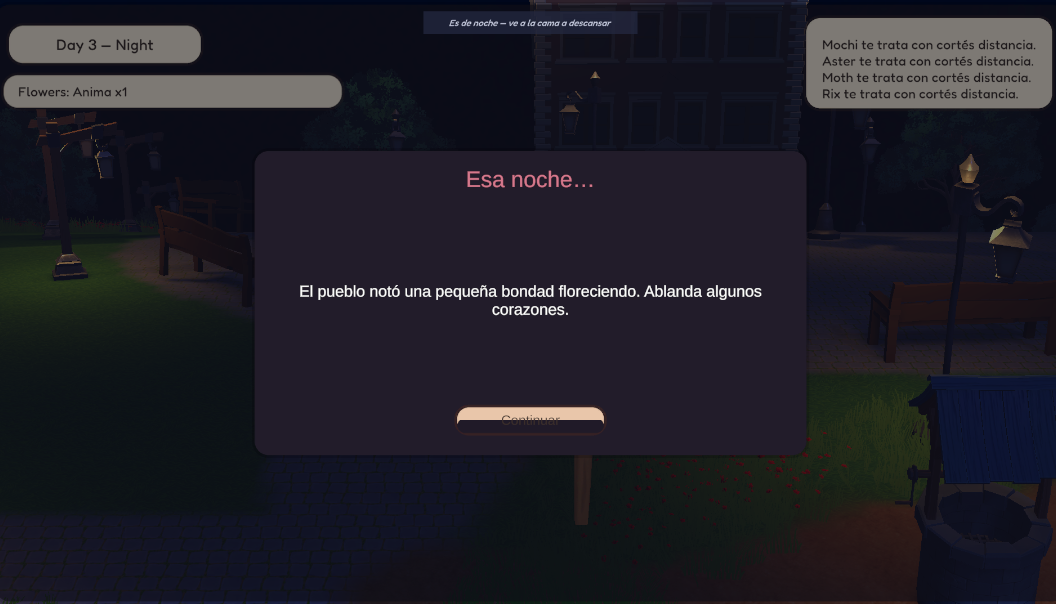
\includegraphics[width=0.5\linewidth]{CotilleoNocturno.png}
    \caption{Enter Caption}
    \label{fig:placeholder}
\end{figure}

\begin{figure}
    \centering
    
\includegraphics[width=0.5\linewidth]{final.png}
    \caption{Enter Caption}
    \label{fig:placeholder}
\end{figure}

\section{Diseño de la evaluación implícita}

El núcleo distintivo de Sprout es su sistema de evaluación implícita: el juego mide pensamiento divergente sin que la jugadora perciba el contexto evaluativo. La medición se restringe deliberadamente a los \textit{nodos de reto creativo} de cada trama (Tabla~\ref{tab:mapeo_ttct}) ---los momentos en que un vecino pide ideas---, dejando fuera saludos y charla cotidiana: las subpruebas del TTCT evalúan producción divergente ante una consigna, no conversación espontánea, y puntuar mensajes sin intención ideativa contaminaría las medidas. La operacionalización de las dimensiones (fluidez, flexibilidad, originalidad, elaboración, y una rúbrica ampliada de cinco dimensiones adicionales que alimentan las mecánicas del juego sin formar parte del marco TTCT) se detalla como implementación técnica en la sección 5.5; baste señalar aquí que, deliberadamente, no se calcula ningún índice compuesto normativo ni «fortalezas creativas» al estilo del TTCT figural, pues eso exigiría baremos poblacionales de los que el prototipo carece y sugeriría una robustez psicométrica que el sistema no reclama (sección 2.2.5).

El feedback a la jugadora nunca es numérico: se comunica por canales diegéticos ---las flores que brotan cada noche (sección 4.6), las frases del resumen nocturno, y el resumen poético del final, que describe el estilo de pensamiento de la partida con imágenes en lugar de puntuaciones («No diste respuestas rápidas. Les pusiste textura, sombra y bordes.»)---. La coherencia con la filosofía de aplicación no amenazante de Torrance (sección 2.2.4) es total: ni siquiera en el desenlace el juego confiesa que ha estado midiendo.

\textcolor{gray}{\textit{[Figura sugerida: diagrama del sistema de estimación (flujo mensaje de la jugadora $\rightarrow$ nodo de reto $\rightarrow$ evaluador LLM $\rightarrow$ perfil por NPC $\rightarrow$ flores / banderas / final), como visión de conjunto de esta sección.]}}

\section{La floristería emocional: mecánica diferencial}

La mecánica diferencial de Sprout ---el rasgo que distingue al juego de cualquier otro proyecto similar--- es la floristería emocional. Cada noche, según las decisiones tomadas durante el día, brotan en el jardín de la florista flores con carga emocional asociada. Al día siguiente, la jugadora combina dos flores para crear ramos con nombre y significado propios, y los regala a los vecinos. El mismo ramo no significa lo mismo para todos los personajes: el sistema de reacciones diferenciales por NPC convierte cada regalo en una decisión narrativa con consecuencias específicas.

El vocabulario de la mecánica son siete flores, cada una asociada a una emoción y a una conducta que la genera (Tabla~\ref{tab:flores}). Las flores no se compran ni se encuentran: brotan como consecuencia, por dos vías. La vía creativa premia el pensamiento divergente observado (fluidez alta hace brotar una flor \textit{Sol}; originalidad alta, una \textit{Acuariana}). La vía narrativa responde a hitos morales de las tramas: la honestidad dolorosa y el rechazo de la mentira generan \textit{Ánima}; cotillear genera \textit{Inquieta}; ayudar a la mentira de Moth genera \textit{Brasa}; un conflicto sin resolver genera \textit{Velada}; una mentira piadosa, \textit{Crisálida}; y que Rix se abra, \textit{Acuariana}. Así, el jardín codifica simultáneamente cómo piensa y cómo actúa la jugadora.

\begin{table}[h]
  \centering
  \caption{Las siete flores emocionales y las conductas que las generan.}
  \label{tab:flores}
  \begin{footnotesize}
  \renewcommand{\arraystretch}{1.3}
  \begin{tabular}{p{2.4cm}p{2.6cm}p{7.6cm}}
    \hline
    \textbf{Flor} & \textbf{Emoción} & \textbf{Conducta generadora} \\
    \hline
    Sol & Alegría & Fluidez alta (muchas ideas concretas en un reto). \\
    \hline
    Acuariana & Calma & Originalidad alta; también, que Rix se abra a la jugadora. \\
    \hline
    Ánima & Honestidad & Honestidad dolorosa; rechazar la mentira de Moth. \\
    \hline
    Crisálida & Secreto & Mentira piadosa a Mochi; guardar un secreto ajeno. \\
    \hline
    Brasa & Pasión & Ayudar a la mentira romántica de Moth. \\
    \hline
    Inquieta & Desasosiego & Cotillear sobre un vecino. \\
    \hline
    Velada & Tristeza & Dejar un conflicto sin resolver. \\
    \hline
  \end{tabular}
  \end{footnotesize}
\end{table}

Sobre ese vocabulario se construye una gramática de ocho ramos, cada uno resultado de combinar dos flores concretas: \textit{Paz} (Sol + Acuariana), \textit{Consuelo} (Velada + Acuariana), \textit{Promesa} (Sol + Ánima), \textit{Confesión} (Crisálida + Ánima), \textit{Obsesión} (Brasa + Inquieta), \textit{Deseo oculto} (Brasa + Crisálida), \textit{Despedida} (Velada + Brasa) y \textit{Sospecha} (Inquieta + Crisálida). Las combinaciones sin receta no producen nada, lo que convierte el crafteo en un pequeño espacio de experimentación. La tabla completa, junto con las reacciones diferenciales de los cuatro vecinos a cada ramo, se recoge en el Anexo E; baste aquí un ejemplo del principio de diferencialidad: el ramo de \textit{Consuelo} hace llorar de gratitud a Mochi, abre a Aster, es malinterpretado por Moth como lástima y ofende a Rix (``no me tengas lástima''), de modo que regalar exige teoría de la mente, no solo inventario.

La justificación académica del bucle decisión-emoción-consecuencia es doble. Por un lado, materializa el tercer pilar de diseño (consecuencia legible) en un objeto persistente y visible ---el jardín--- sin recurrir a métricas, sosteniendo la invisibilidad de la evaluación. Por otro, cierra el circuito conductual que la evaluación implícita necesita: la conducta creativa y moral genera flores, las flores habilitan decisiones nuevas (qué ramo crear, a quién regalarlo), y esas decisiones vuelven a generar conducta observable. La mecánica diferencial no es un adorno sobre el sistema de medida: es su interfaz.

\textcolor{gray}{\textit{[Figuras sugeridas: (1) captura de la estación de creación de ramos con el inventario de flores; (2) lámina con las siete flores y sus nombres (arte del juego); (3) captura de un vecino reaccionando a un ramo.]}}


\section{Diseño de la experiencia: estructura, ritmo y mecánicas}

Las secciones anteriores han descrito los componentes del diseño por separado. Esta sección los integra desde el punto de vista de la jugadora: cómo se estructura una partida, con qué ritmo avanza y qué mecánicas la componen. El objetivo es ofrecer una visión de conjunto del juego antes de entrar, en el Capítulo V, en su implementación técnica.

\subsection{La estructura por fases como esqueleto de la experiencia}

Sprout no se organiza en niveles espaciales al uso, sino en una estructura temporal que cumple la misma función: el \textbf{día dividido en cuatro fases} ---mañana, mediodía, tarde y noche--- actúa como el esqueleto que segmenta y dosifica la experiencia. Cada fase es una unidad rítmica con su propio propósito: las fases diurnas (mañana, mediodía, tarde) son de exploración y conversación con los vecinos, mientras que la noche es un cierre distinto ---no jugable de la misma manera--- en el que los vecinos conversan entre sí (cotilleo) y, al dormir, se cierra el día y se avanza al siguiente. Una partida abarca un número reducido de días (tres por defecto), lo que mantiene la duración total en torno a los quince minutos y convierte cada decisión en algo con peso, al no haber tiempo para deshacerla.

Este esqueleto temporal es también el que gobierna la progresión narrativa: las banderas y contadores acumulados durante las fases diurnas condicionan lo que ocurre de noche y, a través de sucesivos días, el desenlace. La fase, por tanto, no es solo una ambientación de la luz, sino la unidad que ordena el ritmo, el contenido disponible y las consecuencias.

\subsection{Entrada a la experiencia: el onboarding}

La primera partida comienza con una secuencia de llegada al pueblo a bordo de un coche, durante la cual un personaje conductor conversa con la protagonista e introduce la premisa ---la floristería que le ha dejado su abuela--- sin recurrir a un tutorial expositivo. A continuación, un breve recorrido guiado presenta los lugares clave (la casa y la floristería). Durante estas secuencias se ocultan los elementos de interfaz no esenciales y se acota el control de la jugadora, de modo que la introducción se perciba como parte de la ficción y no como una pantalla de ayuda. El diseño del onboarding busca así enseñar a jugar mostrando, coherente con la filosofía no expositiva del proyecto.

\begin{figure}
    \centering
    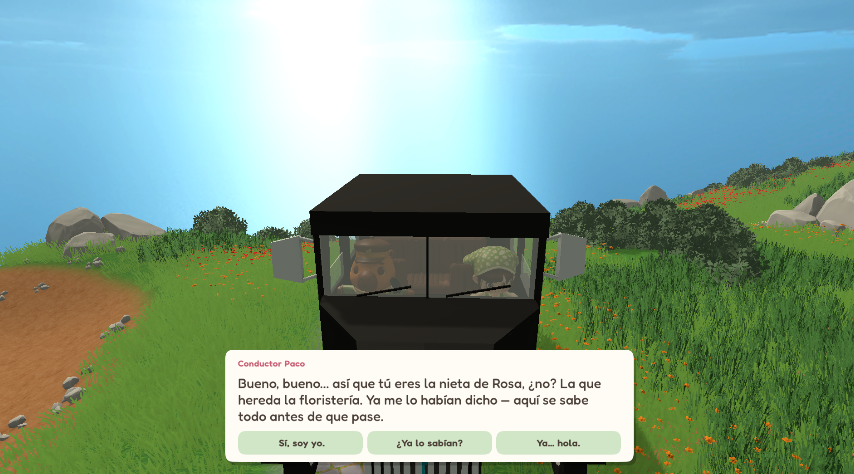
\includegraphics[width=0.5\linewidth]{intro.png}
    \caption{Enter Caption}
    \label{fig:placeholder}
\end{figure}

\begin{figure}
    \centering
    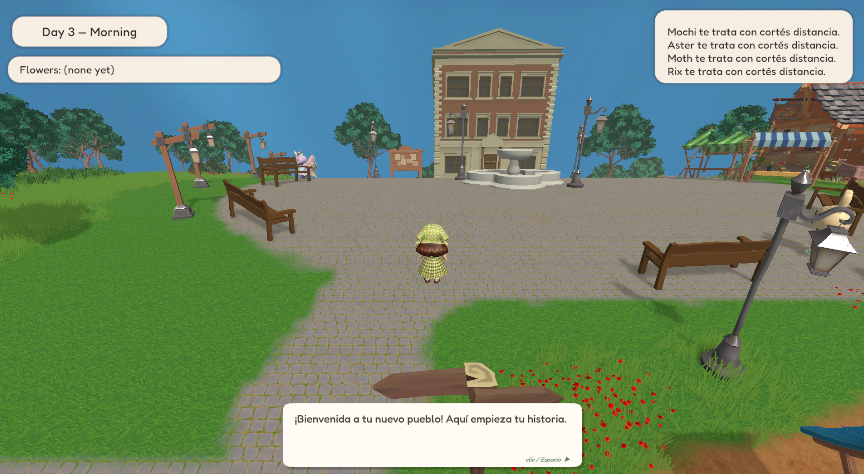
\includegraphics[width=0.5\linewidth]{image.png}
    \caption{Enter Caption}
    \label{fig:placeholder}
\end{figure}
\subsection{El bucle jugable}

Dentro de cada fase diurna, la jugadora repite un bucle sencillo: explora el pueblo y entra en las casas; conversa con un vecino a través del sistema de diálogo, que combina tramos guionizados con conversación abierta gobernada por IA; en los momentos de reto, sus respuestas alimentan ---de forma invisible--- la evaluación de creatividad (sección 4.5); como consecuencia de sus decisiones y de su creatividad, obtiene flores emocionales que brotan en el macetero; combina flores en ramos y los regala, provocando reacciones diferentes en cada vecino (sección 4.6); y esas acciones modifican relaciones y banderas que se propagarán por la noche. Al dormir, el día se cierra, se guarda la partida y comienza el siguiente. El bucle es deliberadamente corto y legible, para que la jugadora perciba con claridad la cadena decisión-emoción-consecuencia que vertebra el juego.

\subsection{La expresión de la jugadora como contexto conversacional}

Antes de escribir, la jugadora puede fijar una expresión facial de su personaje ---por ejemplo, enfadada o ilusionada--- tocando su propio retrato en la interfaz de diálogo; el gesto elegido persiste hasta que elige otro. La elección no es solo cosmética: la etiqueta de la expresión se añade como contexto al mensaje que recibe la IA («la florista te dice esto con expresión/tono enfadada»), de modo que el vecino puede reaccionar al gesto además de al contenido de lo dicho, igual que haría cualquiera al notar la cara de quien le habla. A esto se suman detalles menores de la misma capa expresiva: la boca se mueve mientras la jugadora escribe su mensaje, y el personaje parpadea automáticamente en los ratos de espera, buscando que la cara comunique tanto como las palabras.

\subsection{Guía de la jugadora sin puntuaciones}

Un principio de diseño transversal es que el juego nunca muestra puntuaciones ni descubre que está midiendo creatividad. La guía se ofrece por medios diegéticos: indicadores luminosos (\textit{glow}) sobre los vecinos comunican su estado o si conviene visitarlos, y el resumen del cotilleo nocturno insinúa las consecuencias de lo ocurrido durante el día. De este modo, la jugadora recibe orientación suficiente para avanzar sin que el sistema rompa la ilusión de estar simplemente conversando y regalando flores.

\subsection{Visión de conjunto de las mecánicas}

La Tabla~\ref{tab:mecanicas} resume las mecánicas que componen la experiencia y remite a la sección donde se detalla su implementación técnica.

\begin{table}[h]
  \centering
  \caption{Mecánicas de Sprout y su ubicación en la memoria.}
  \label{tab:mecanicas}
  \begin{footnotesize}
  \renewcommand{\arraystretch}{1.3}
  \begin{tabular}{p{3.6cm}p{7.4cm}p{2cm}}
    \hline
    \textbf{Mecánica} & \textbf{En qué consiste} & \textbf{Detalle} \\
    \hline
    Exploración y movimiento & Recorrer el pueblo y entrar en las casas; cámara en tercera persona en los interiores. & Cap. V \\
    \hline
    Diálogo ramificado con IA & Conversar con los vecinos combinando tramos guionizados y conversación abierta gobernada por un LLM. & Sec. 4.4, 5.3--5.5 \\
    \hline
    Evaluación implícita de creatividad & Puntuar de forma invisible el pensamiento divergente de la jugadora en los nodos de reto. & Sec. 4.5, 5.5 \\
    \hline
    Expresiones faciales & Fijar un gesto de la protagonista que persiste y condiciona la respuesta del vecino. & Cap. V \\
    \hline
    Floristería emocional & Obtener flores, combinarlas en ramos y regalarlas, con reacciones diferenciales por vecino. & Sec. 4.6, 5.7 \\
    \hline
    Macetero & Las flores obtenidas crecen como modelos 3D en el jardín, como registro visual del avance. & Sec. 5.7 \\
    \hline
    Cotilleo nocturno & De noche, los vecinos propagan información entre sí y alteran relaciones y banderas. & Sec. 4.4 \\
    \hline
    Relaciones y finales múltiples & El estado acumulado de relaciones y banderas determina el desenlace de la partida. & Sec. 4.4 \\
    \hline
    Guardado al dormir & Dormir cierra el día y guarda el estado completo de la partida. & Sec. 5.9 \\
    \hline
  \end{tabular}
  \end{footnotesize}
\end{table}

En conjunto, estas mecánicas no son módulos independientes yuxtapuestos, sino piezas de un mismo bucle: la conversación alimenta la creatividad y la narrativa, estas generan flores y consecuencias, las flores y las decisiones alteran las relaciones, y las relaciones ---propagadas por el cotilleo--- reconfiguran las conversaciones del día siguiente. El grafo de diálogo, descrito como eje técnico en el Capítulo V, es el sustrato sobre el que este bucle se articula.

\textcolor{gray}{\textit{[Figura sugerida: diagrama del sistema completo (el «diagrama del sistema» del juego): los subsistemas ---diálogo, IA conversacional, estimación de creatividad, flores, cotilleo, relaciones, finales, guardado--- como cajas, con flechas que muestren el bucle descrito en este párrafo.]}}

\chapter{Implementación técnica}

Este capítulo describe la implementación técnica del prototipo Sprout en Unity 6. La arquitectura adopta principios de arquitectura limpia por capas adaptados al entorno Unity mediante ScriptableObjects (Hipple, 2017), con una separación clara entre lógica de dominio, lógica de aplicación, infraestructura y presentación. La comunicación entre módulos se realiza mediante un sistema de eventos basado en ScriptableObjects que mantiene los componentes desacoplados y testeables. El capítulo se organiza siguiendo las capas y módulos principales del sistema, desde la arquitectura general hasta el pipeline de renderizado.
\section{Arquitectura del sistema}

La regla de oro de la arquitectura de Sprout es esta: \textbf{las reglas del juego no deben saber que existe una pantalla, un botón o una API externa}. Si mañana cambiase todo el aspecto visual del juego, las reglas de qué ramo gusta a qué vecino no deberían tocarse ni una línea. Para conseguirlo, el proyecto se organiza en cuatro carpetas, cada una con un trabajo distinto:

\begin{itemize}
  \item \textbf{\texttt{0.Core} (dominio)} --- C\# puro, sin ninguna dependencia de \texttt{UnityEngine}: el perfil de creatividad (\texttt{CreativityProfile}), el resolutor de ramos (\texttt{BouquetResolver}), el motor de cotilleo (\texttt{GossipRuleEngine}), el resolutor de finales (\texttt{EndingResolver}), el ciclo de día (\texttt{DayCycleState}) y el almacén de banderas narrativas (\texttt{NarrativeFlagStore}).
  \item \textbf{\texttt{1.Application}} --- quien dirige la partida usando esas reglas: el director de juego (\texttt{SproutGameDirector}), los servicios de día, flores y finales, y el cerebro conversacional de los NPCs.
  \item \textbf{\texttt{2.Infraestructure}} --- los detalles externos: el cliente de la API de OpenAI, la persistencia en disco y el sistema de eventos.
  \item \textbf{\texttt{3.Presentation}} --- lo que se ve y se toca: cámaras, animación, interfaz, interacción, efectos visuales.
\end{itemize}

Esta regla no es solo una intención de diseño, sino algo que \textbf{Unity impone técnicamente} mediante una Assembly Definition: un archivo de configuración que convierte una carpeta en un bloque de compilación aislado, separado del resto del proyecto. En Sprout, la carpeta \texttt{0.Core/Domain} tiene una de estas fronteras (\texttt{Sprout.Domain.asmdef}), con dos propiedades relevantes: no depende de ningún otro bloque del proyecto, y tiene activada la opción \texttt{noEngineReferences}, que prohíbe expresamente el uso de \texttt{UnityEngine} dentro de esa carpeta. La consecuencia práctica es que el resto del proyecto (Application, Infraestructure, Presentation) puede usar el código del dominio con normalidad, pero el dominio nunca puede usar nada de fuera: si alguien escribiera por error una línea de código de Unity dentro de esa carpeta, el proyecto sencillamente no compilaría (Figura~\ref{fig:asmdef-direccion}). La dependencia, por tanto, solo circula en un sentido.

Frente al patrón Singleton habitual en proyectos Unity ---donde cualquier script accede a \texttt{Manager.Instance} desde cualquier punto del código---, Sprout modela la configuración y los canales de comunicación como ScriptableObjects. La crítica de Hipple (2017) al Singleton señala tres problemas concretos, y los tres tienen su contrapartida aplicada en el proyecto. Primero, las conexiones rígidas rompen la modularidad, porque un sistema no puede existir sin arrastrar a todos los que dependen de él; en Sprout esto se evita con el sistema de eventos desacoplado, detallado en la sección 5.5. Segundo, el Singleton elimina el polimorfismo, porque \texttt{Instance} siempre devuelve el mismo tipo concreto y no permite sustituirlo por una versión de prueba; en Sprout, \texttt{AISettingsSO} resuelve justo este problema para el módulo de IA, incorporando un modo simulado que sustituye las llamadas reales a la API sin tocar el código que las consume (sección 5.3). Tercero, el Singleton provoca condiciones de carrera en el arranque, porque un objeto puede referenciarse antes de que su manager exista; los ScriptableObjects evitan esto porque su copia en memoria está disponible en cuanto se referencian, sin depender de que ningún \texttt{Awake} se haya ejecutado antes. En los tres casos, el Inspector de Unity hace de inyector de dependencias: cualquier componente arrastra la referencia al activo que necesita, sin buscarlo en la escena ni depender de una instancia global.

\begin{sloppypar}
Debe señalarse una excepción consciente a este mismo principio: \texttt{SproutGameDirector} sí se implementa como una instancia estática accesible globalmente (\texttt{.Instance}), reintroduciendo precisamente el riesgo de condición de carrera en el arranque descrito arriba. La decisión es pragmática: el estado de una partida ---banderas, relaciones, inventario, día actual--- es, por naturaleza, una única cosa compartida por todo el juego durante toda la sesión; no existen dos partidas simultáneas ni dos \texttt{SproutGameDirector}, así que el riesgo de condición de carrera se limita a un único punto de arranque, no a una cadena de managers dependientes entre sí. Montar la infraestructura de ScriptableObject inyectado para una instancia que nunca va a duplicarse no aporta ninguna ventaja real en este proyecto. El propio Hipple (2017) admite que el patrón resulta razonable en casos puntuales de estado genuinamente único; lo que sí se evitó fue encadenar singletons unos sobre otros ---el error que el autor señala como el más costoso---, delegando en ScriptableObjects el resto de la comunicación entre sistemas.
La Figura~\ref{fig:gsm-inspector} lo muestra de forma directa sobre el propio proyecto: el componente \texttt{Game State Machine}, adjunto al objeto \texttt{GameManager}, es en sí mismo una instancia única y accesible globalmente (\texttt{.Instance}), pero cada uno de sus seis campos de evento ---\texttt{Ev\_EnterMainMenu}, \texttt{Ev\_EnterLoading}, \texttt{EV\_EnterPlaying}, \texttt{EV\_EnterPaused}, \texttt{EV\_ResumePlaying}, \texttt{Ev\_EnterEnding}--- apunta a un activo \texttt{Game Event SO} distinto. El propio Inspector deja ver la convivencia de los dos patrones: el Singleton resuelve "que solo exista una máquina de estados y cualquier script pueda encontrarla"; los ScriptableObjects resuelven "que, cuando cambie de estado, se enteren los sistemas interesados sin que la máquina de estados necesite conocerlos". Ninguno de los seis eventos es una referencia directa a otro objeto de la escena: son activos del proyecto, sustituibles y observables desde el propio Inspector, tal y como muestra la captura.
\end{sloppypar}

\begin{figure}[H]
    \centering
    \includegraphics[width=1\linewidth]{gamemanager_inspector.png}
    \caption{Inspector del objeto \texttt{GameManager}, mostrando el componente \texttt{Game State Machine} y sus seis eventos de estado, cada uno un activo \texttt{Game Event SO} independiente.}
    \label{fig:gsm-inspector}
\end{figure}

\begin{sloppypar}
Por último, las fronteras entre capas se abstraen mediante interfaces ---\texttt{ISettingsRepository} (persistencia de ajustes), \texttt{ISceneLoader} (carga de escenas), \texttt{IInteractable} (objetos interactuables) e \texttt{IPlayerController} (control del personaje)---, de modo que la capa de presentación y la de infraestructura pueden sustituirse sin tocar la lógica que depende de ellas.
\end{sloppypar}


\begin{figure}[H]
    \centering
    \begin{tikzpicture}[
        box/.style={draw, rounded corners, minimum width=4.4cm, minimum height=1.1cm, align=center, font=\small},
        node distance=0.55cm
    ]
        \node[box, fill=orange!10] (pres) {3. Presentation};
        \node[box, fill=orange!10, below=of pres] (infra) {2. Infraestructure};
        \node[box, fill=orange!10, below=of infra] (app) {1. Application};
        \node[box, fill=blue!15, below=of app, minimum height=1.4cm, yshift=-0.9cm] (dom) {\texttt{0.Core} (\texttt{Sprout.Domain})\\ \footnotesize \texttt{noEngineReferences: true}};

        \draw[dashed, thick] ($(pres.north west)+(-0.3,0.3)$) rectangle ($(app.south east)+(0.3,-0.3)$);
\node[font=\footnotesize, anchor=south] at ($(pres.north)+(0,0.35)$) {mismo ensamblado (\texttt{Assembly-CSharp})};
        \draw[-{Latex[length=3mm]}, thick] (app.south) -- (dom.north);
        \node[font=\footnotesize, fill=white, inner sep=1pt] at ($(app.south)!0.5!(dom.north)$) {puede usar};
    \end{tikzpicture}
    \caption{Solo el dominio (\texttt{0.Core}) tiene un ensamblado propio impuesto por Unity; las otras tres capas comparten el mismo ensamblado y se separan solo por convención de carpetas.}
    \label{fig:capas-ensamblados}
\end{figure}

\begin{figure}[H]
    \centering
       \begin{tikzpicture}[
        c/.style={draw, rounded corners, minimum width=3.4cm, minimum height=0.9cm, align=center, font=\footnotesize},
        >=Latex
    ]
        \node[c, fill=orange!10] (api) at (-6,3.2) {OpenAIApi};
        \node[c, fill=orange!10] (ss)  at (0,3.2) {SaveSystem};

        \node[c, fill=green!10] (npc) at (-6,1.1) {NPCBrain};
        \node[c, fill=green!10] (ct)  at (-6,-1.1) {CreativityTracker};
        \node[c, fill=green!10, minimum width=4cm] (sgd) at (0,0) {SproutGameDirector};
        \node[c, fill=green!10] (fs)  at (6,1.1) {FlowerService};
        \node[c, fill=green!10] (ngs) at (6,-1.1) {NightGossipService};
        \node[c, fill=green!10] (es)  at (6,-2.9) {EndingService};

        \node[c, fill=blue!10] (cp)  at (-6,-4.4) {CreativityProfile};
        \node[c, fill=blue!10] (dc)  at (-2,-4.4) {DayCycleState};
        \node[c, fill=blue!10] (gre) at (2,-4.4) {GossipRuleEngine};
        \node[c, fill=blue!10] (er)  at (6,-4.4) {EndingResolver};

        \draw[->] (npc) -- (api);
        \draw[->] (ct) -- (npc);
        \draw[->] (ct) -- (sgd);
        \draw[->] (fs) -- (sgd);
        \draw[->] (ss) -- (sgd);
        \draw[->] (sgd) -- (cp);
        \draw[->] (sgd) -- (dc);
        \draw[->] (ngs) -- (sgd);
        \draw[->] (ngs) -- (gre);
        \draw[->] (es) -- (sgd);
        \draw[->] (es) -- (er);
    \end{tikzpicture}
    \caption{Relaciones verificadas entre las clases principales. \texttt{SproutGameDirector} actúa como centro que la mayoría de servicios de aplicación consultan mediante \texttt{.Instance}; el dominio (azul) solo recibe llamadas, nunca las hace.}
    \label{fig:clases-generales}
\end{figure}


\section{Sistema de estados --- HFSM}

El estado del juego y del jugador se gestiona mediante una máquina de estados finitos jerárquica (HFSM) que separa flujos macro (del juego completo) y flujos micro (del personaje jugador). Esta separación evita el anti-patrón de las máquinas de estado planas, cuya cantidad de transiciones crece de forma combinatoria al mezclar estados de niveles distintos.

En el nivel macro, la \texttt{GameStateMachine} gobierna el ciclo de vida de la aplicación con cinco estados: \textit{Boot} (arranque e inicialización de servicios), \textit{MainMenu}, \textit{Playing}, \textit{Paused} y \textit{Ending} (pantalla de desenlace). Las transiciones se anuncian mediante eventos de juego (sección 5.6), de modo que los sistemas interesados ---la pantalla de carga, que se oculta al entrar en \textit{Playing}; el propio jugador, que se bloquea al entrar en \textit{Paused}--- reaccionan sin acoplarse a la máquina. La carga de escenas no es un estado propio sino una responsabilidad delegada en la abstracción \texttt{ISceneLoader}, cuya implementación (\texttt{SceneLoader}) muestra la pantalla de carga durante las transiciones; la entrada de pausa se captura en un manejador dedicado (\texttt{PauseInputHandler}) que solicita la transición en lugar de ejecutarla.

En el nivel micro, la \texttt{PlayerStateMachine} gestiona el comportamiento del personaje con cuatro estados que heredan de una base común (\texttt{PlayerBaseState}): \textit{FreeRoam} (exploración con movimiento), \textit{Dialogue} (control cedido a la conversación: el movimiento se bloquea y la cámara encuadra al interlocutor), \textit{Inspect} (examinar objetos, como las cartas de la abuela) y \textit{Paused}. Cada estado encapsula su gestión de entrada y sus condiciones de salida, de modo que añadir un estado nuevo no exige revisar los existentes. Los NPCs disponen de su propia máquina ligera (\texttt{NPCStateMachine}) que alterna entre deambular por el pueblo e interactuar con la jugadora.

\begin{sloppypar}
A diferencia de las transiciones de \texttt{GameStateMachine}, las de \texttt{PlayerStateMachine} no se anuncian mediante eventos ScriptableObject: pasar de \textit{FreeRoam} a \textit{Dialogue} es una decisión que el propio jugador toma sobre sí mismo, no la comunicación entre dos sistemas que no se conocen, así que desacoplarla no aportaría nada. La excepción es la pausa, que sí llega desde fuera ---la dispara \texttt{GameStateMachine}---, y por eso \texttt{EnterPaused()} y \texttt{ResumeFromPause()} se invocan mediante \texttt{GameEventListener}, igual que en el resto de sistemas descritos en la sección 5.5.
\end{sloppypar}

La justificación de la jerarquía es clásica: sin ella, estados compuestos como ``jugando pero en diálogo y luego pausado'' obligarían a duplicar transiciones en una máquina plana; con ella, la pausa global y el estado local del jugador evolucionan por separado y se componen.

\begin{figure}[H]
\centering
\resizebox{\linewidth}{!}{%
\begin{tikzpicture}[
  >={Stealth[length=2.5mm]},
  state/.style={draw, rounded corners=3pt, thick, fill=gray!8,
    minimum width=2.6cm, minimum height=1cm, align=center, font=\small},
  lbl/.style={font=\scriptsize, align=center, fill=white, inner sep=1pt}
]
\node[state] (boot) {Boot};
\node[state, right=2.6cm of boot] (menu) {MainMenu};
\node[state, right=2.6cm of menu] (playing) {Playing};
\node[state, below=1.6cm of playing] (paused) {Paused};
\node[state, right=2.6cm of playing] (ending) {Ending};

\draw[->] (boot) -- (menu) node[lbl, midway, above] {init OK};
\draw[->] (menu) to[bend left=15] node[lbl, above] {StartGame()\\(chequeo IA OK)} (playing);
\draw[->, dashed] (playing) to[bend left=15] node[lbl, below] {chequeo IA falla} (menu);
\draw[->] ($(playing.south)+(-0.3,0)$) to[bend right=12] node[lbl, left] {Ev\_EnterPaused} ($(paused.north)+(-0.3,0)$);
\draw[->] ($(paused.north)+(0.3,0)$) to[bend right=12] node[lbl, right] {Ev\_ResumePlaying} ($(playing.south)+(0.3,0)$);
\draw[->] (playing) -- (ending) node[lbl, midway, above] {condición\\de final};
\end{tikzpicture}%
}
\caption{Transiciones de la GameStateMachine (macro-FSM). El paso de MainMenu a Playing solo ocurre si el chequeo de conexión con la IA es correcto; si falla, se vuelve a MainMenu. Paused y Ending se superponen sin recargar escena.}
\label{fig:hfsm-gamestate}
\end{figure}


\begin{figure}[H]
\centering
\begin{tikzpicture}[
  >={Stealth[length=2.5mm]},
  state/.style={draw, rounded corners=3pt, thick, fill=gray!8,
    minimum width=2.8cm, minimum height=1cm, align=center, font=\small},
  lbl/.style={font=\scriptsize, align=center, fill=white, inner sep=1pt}
]
\node[state] (free) {FreeRoam\\\footnotesize(inicial)};
\node[state, above right=1.8cm and 3.2cm of free] (dialogue) {Dialogue};
\node[state, below right=1.8cm and 3.2cm of free] (inspect) {Inspect};
\node[state, right=6.6cm of free] (paused) {Paused};

\draw[->] ($(free.north)+(0.15,0)$) to[bend left=10] node[lbl, above] {EnterDialogue()} ($(dialogue.west)+(0,-0.12)$);
\draw[->] ($(dialogue.west)+(0,0.12)$) to[bend left=10] node[lbl, below] {EnterFreeRoam()} ($(free.north)+(-0.15,0)$);
\draw[->] ($(free.south)+(0.15,0)$) to[bend right=10] node[lbl, below] {EnterInspect()} ($(inspect.west)+(0,0.12)$);
\draw[->] ($(inspect.west)+(0,-0.12)$) to[bend right=10] node[lbl, above] {EnterFreeRoam()} ($(free.south)+(-0.15,0)$);
\draw[->, dashed] (dialogue.east) to[bend left=8] node[lbl, above] {Ev\_EnterPaused\\(guarda estado)} (paused.north);
\draw[->, dashed] (inspect.east) to[bend right=8] node[lbl, below] {Ev\_EnterPaused\\(guarda estado)} (paused.south);
\draw[->, dashed] (free.east) to node[lbl, above, pos=0.35] {Ev\_EnterPaused} (paused.west);
\draw[->] (paused.south) to[out=-90, in=-90, looseness=2.4] node[lbl, below, pos=0.5] {Ev\_ResumePlaying\\(restaura estado anterior)} (free.south);
\end{tikzpicture}
\caption{Transiciones de la PlayerStateMachine (micro-FSM). Pausa "apilable": desde cualquier estado se guarda cuál era el estado activo, y al reanudar se vuelve exactamente a ese mismo estado (no siempre a FreeRoam).}
\label{fig:hfsm-player}
\end{figure}

\subsection{Modelo de datos: el grafo y los nodos}
El grafo se representa mediante el ScriptableObject \texttt{DialogueGraphSO}, que almacena la lista de nodos que lo componen, una referencia al nodo de entrada y las posiciones de cada nodo en el lienzo del editor. El nodo de entrada, además, no se marca a mano: al guardar el grafo, la herramienta recorre todas las conexiones y designa como entrada al único nodo que no recibe ninguna arista entrante. El empleo de ScriptableObjects es deliberado: son el mecanismo de serialización propio de Unity y permiten que el contenido narrativo se gestione como un recurso del proyecto, independiente de las escenas.

Todos los nodos derivan de la clase abstracta \texttt{DialogueNodeSO}, que reúne los atributos comunes a cualquier momento de la conversación: un identificador único (\texttt{nodeGuid}), el contexto que se transmite a la inteligencia artificial en ese punto (\texttt{contextForAI}), las condiciones de acceso (\texttt{prerequisiteFlags}), los cambios de estado que se aplican al entrar (\texttt{flagsOnEnter}), una respuesta alternativa para cuando no se cumplen los requisitos (\texttt{lockedReply}) y la lista de nodos siguientes. Cada nodo puede definir también una \texttt{resumeLine}: una frase de bienvenida distinta que se muestra si la jugadora abandona la conversación a medias y vuelve más tarde, en lugar de repetir siempre la misma frase inicial. Sobre esta base se definen tres tipos concretos de nodo, resumidos en la Tabla~\ref{tab:tipos_nodo}.

\begin{table}[h]
  \centering
  \caption{Tipos de nodo del sistema de diálogo.}
  \label{tab:tipos_nodo}
  \begin{footnotesize}
  \renewcommand{\arraystretch}{1.3}
  \begin{tabular}{p{2.6cm}p{6cm}p{4.5cm}}
    \hline
    \textbf{Tipo de nodo} & \textbf{Comportamiento} & \textbf{Campos propios} \\
    \hline
    SpeechNode & El NPC pronuncia una línea y la conversación avanza sola al siguiente nodo; si hay varios nodos siguientes posibles, se elige el primero cuyas banderas de acceso se cumplan. & Frase inicial; lista de nodos siguientes. \\
    \hline
    ChoiceNode & Punto de ramificación mediante texto libre: el NPC plantea la situación y la jugadora responde escribiendo con sus propias palabras, sin botones. Una llamada aparte a la IA clasifica esa respuesta contra una lista de condiciones en lenguaje natural y dirige la conversación a la rama correspondiente. & Frase inicial; lista de opciones, cada una con una condición en lenguaje natural y un nodo destino. \\
    \hline
    ConversationNode & Conversación abierta sobre varios temas dentro del mismo nodo; no se ramifica. Solo avanza cuando la IA determina, tras cada mensaje, que se cumple una condición de salida expresada en lenguaje natural. & Frase inicial; temas de conversación; condición de salida. \\
    \hline
  \end{tabular}
  \end{footnotesize}
\end{table}

La distinción entre el ChoiceNode y el ConversationNode es la que mejor ilustra la filosofía del sistema, y ambos comparten un rasgo clave: en ninguno de los dos elige la jugadora de un menú, sino que escribe libremente y es la IA quien decide, contra un criterio en lenguaje natural definido en el propio nodo, hacia dónde avanza la historia. El ChoiceNode acota ese criterio a un conjunto cerrado de destinos posibles (una condición por rama); el ConversationNode, en cambio, no tiene ramas: solo comprueba, mensaje a mensaje, si ya se puede dar por cerrado el tema y pasar al siguiente nodo.

\revisar{el grafo de mochi no me convence, si lo cambio cambiar este texto}
Un ejemplo real del proyecto, tomado directamente del nodo \texttt{Mochi\_taste} (\texttt{ChoiceNodeSO}): el contexto que recibe la IA es \textit{``TARDE. Mochi ofrece un risotto experimental amargo y espera reacción. Decisión clave del jugador: honestidad con tacto, mentira amable, crueldad, o evasiva''}, y sus cuatro opciones no llevan texto de botón alguno, solo una condición y un destino, por ejemplo \textit{``el jugador es honesto con tacto (dice que no está bueno sin ser cruel)''} o \textit{``el jugador es cruel o se burla de la comida''}. La jugadora simplemente escribe lo que le diría a Mochi, y la IA decide cuál de las cuatro ramas describe mejor su respuesta.
\revisar{poner aqui una foto}

\subsection{Puertas narrativas y banderas de estado}
El control del progreso narrativo se realiza mediante banderas (flags) booleanas. Cada nodo puede declarar una lista de requisitos previos, donde cada requisito asocia el nombre de una bandera con el valor esperado. Antes de permitir el acceso a un nodo, el sistema comprueba que todas las banderas requeridas tengan el valor previsto; si no es así, el nodo permanece bloqueado y se devuelve la respuesta definida para ese caso. De manera complementaria, un nodo puede activar banderas al ser alcanzado, lo que permite que la historia registre que la jugadora ha pasado por un determinado momento y desbloquee, en consecuencia, contenidos posteriores.

Esta misma comprobación de banderas es también el mecanismo de ramificación de los SpeechNode: un nodo puede tener más de un nodo siguiente candidato, y el motor recorre la lista en orden y elige el primero cuyas banderas se cumplan (con un último candidato sin requisitos a modo de ``en caso contrario''). Esto permite bifurcar la historia según el estado acumulado del juego, sin necesidad de que la jugadora tome ninguna decisión explícita en ese punto. Este mecanismo convierte el grafo en una máquina narrativa con memoria de estado, cuyas banderas alimentan además el sistema de cotilleos nocturnos y la resolución del final.
\revisar{poner aqui una foto}

\subsection{El editor visual basado en GraphView}
El editor se materializa en una ventana de editor accesible desde el menú de herramientas de Unity, que ofrece acciones para guardar y cargar grafos. El lienzo proporciona las manipulaciones habituales de un editor de grafos ---zoom, desplazamiento, rejilla de fondo y selección por rectángulo--- y responde a la petición de creación de nodos abriendo un buscador que permite insertar cualquiera de los tres tipos de nodo en la posición del cursor. Cada nodo se dibuja codificando su tipo por color ---azul para Speech, marrón para Choice y verde para Conversation---, lo que facilita la lectura del grafo de un vistazo. Dentro de cada caja se exponen, de forma editable en línea, los campos relevantes del nodo.

Las conexiones se establecen a través de puertos: cada nodo dispone de un puerto de entrada de capacidad múltiple y, salvo los ChoiceNode, de un único puerto de salida que también admite varias conexiones a la vez ---el soporte visual del ramificado por banderas descrito en la sección anterior---. Los ChoiceNode, en cambio, generan un puerto de salida independiente y de conexión única por cada opción, de modo que cada rama de la elección se traza visualmente por separado y queda inequívocamente asociada a su condición.

\textcolor{gray}{\textit{[Figura sugerida (imprescindible): captura del editor de grafos con un diálogo real abierto, donde se aprecien los tres tipos de nodo por color, los puertos y varias conexiones. Es la imagen que mejor demuestra la herramienta propia del proyecto.]}}
\revisar{poner aqui una foto}
\subsection{Serialización y persistencia}

La persistencia del grafo se resuelve sin definir ningún formato propio, aprovechando que los ScriptableObjects ya son serializados por Unity a ficheros de texto. La responsabilidad del serializador se limita, por tanto, a decidir qué objetos se almacenan y a traducir la representación visual ---nodos y aristas--- al modelo de datos. Durante el guardado, el serializador parte de un estado limpio y, por cada caja presente en el lienzo, incrusta su ScriptableObject dentro del propio fichero del grafo mediante \texttt{AddObjectToAsset}. Esta técnica de sub-activos es la decisión central del mecanismo: permite que un grafo completo, con todos sus nodos, resida en un único fichero, evitando la proliferación de archivos sueltos. A cada nodo se le asigna un identificador único y su posición se registra en una lista paralela emparejada por ese identificador, de manera que al reabrir el grafo cada caja recupere su ubicación. Seguidamente, las aristas se traducen a referencias entre nodos ---por puerto en el caso de los ChoiceNode---, y el nodo de entrada se deduce automáticamente como aquel que no recibe ninguna arista. Un aspecto arquitectónicamente relevante es que el editor y el motor de juego comparten exactamente los mismos ScriptableObjects: lo que se dibuja en el editor es, literalmente, lo que el juego recorre en tiempo de ejecución, lo que elimina una posible fuente de discrepancias entre la herramienta de autoría y el comportamiento real.
\begin{figure}
    \centering
    \includegraphics[width=1\linewidth]{grafos_nodos.png}
    \caption{Enter Caption}
    \label{fig:placeholder}
\end{figure}

\subsection{Ejecución en tiempo de juego}

En tiempo de ejecución, el componente DialogueRunner se encarga de recorrer el grafo. Al iniciar una conversación con un NPC, comprueba si ya existe una conversación a medias con él: si es la primera vez (o si ya se encontraba exactamente en el nodo de entrada), reinicia el historial de la IA y sitúa la conversación en el nodo de entrada que corresponda al día y la franja horaria actuales, resuelto por un enrutador dedicado (DialogueEntryRouter). Si, en cambio, la jugadora abandonó la charla a medio camino, el runner retoma exactamente el nodo en el que se quedó, sin reiniciar el historial, de modo que el personaje "recuerda" el hilo de la conversación. Este punto de la conversación se persiste además en el sistema de guardado: cada NPC almacena el identificador del nodo en el que se quedó, y al cargar la partida el runner lo restaura, de forma que retomar una charla sobrevive incluso a cerrar el juego.

Por cada mensaje de la jugadora, el runner delega en el cerebro conversacional la decisión de avanzar o no de nodo y, una vez procesado el turno, emite un evento que comunica el nodo en el que ha quedado la conversación. Este evento es el punto de enganche que permite a otros sistemas —en particular, al evaluador de creatividad— reaccionar a la evolución del diálogo sin acoplarse directamente a él.

\subsection{Integración con la IA conversacional y la evaluación}

º   La herramienta de grafos no es un módulo aislado, sino el sustrato sobre el que operan el resto de sistemas conversacionales. El contexto de cada nodo se incorpora al mensaje de sistema que se envía al modelo de lenguaje, de modo que la inteligencia artificial dispone en todo momento del contexto narrativo del punto exacto en que se encuentra la conversación. Asimismo, el evento de avance alimenta al rastreador de creatividad, que solo evalúa los mensajes emitidos mientras la conversación permanece en el nodo de ideas designado. De esta forma, el grafo determina cuándo y bajo qué contexto se produce ---y se mide--- la actividad de pensamiento divergente, lo que justifica que esta herramienta constituya el eje técnico del proyecto.

\section{Sistema de IA conversacional con memoria}

Cada NPC de Sprout está gobernado por un módulo conversacional (\texttt{NPCBrain}) que combina un perfil de personalidad estático (definido como ScriptableObject) con una memoria dinámica y el contexto narrativo del momento. El módulo se comunica con la API de OpenAI a través de una capa de abstracción (\texttt{OpenAIApi}, en la capa de infraestructura) que aísla al resto del sistema de los detalles de transporte HTTP, autenticación y formato de respuesta. La clave de API nunca se incrusta en el proyecto: se resuelve en tiempo de ejecución desde una variable de entorno, un fichero en StreamingAssets o la configuración local del usuario, y el resto de parámetros ---modelos empleados, tiempos de espera, modo simulado para pruebas sin red--- residen en un ScriptableObject de configuración (\texttt{AISettingsSO}).

La personalidad de cada vecino se define como un activo \texttt{CharacterProfileSO} con cuatro campos de autoría: la \textit{persona} (quién es y cómo se comporta), el \textit{conocimiento del mundo} (lo que sabe de su rincón del pueblo y de su situación actual), el \textit{estilo de habla} y una lista de \textit{reglas obligatorias} propias, junto con un límite máximo de palabras por réplica que preserva el ritmo de juego. La Tabla~\ref{tab:perfiles} resume los cuatro perfiles; su contenido completo se recoge en el Anexo A.
\revisar{no me gustan mucho los perfiles si da tiempo los actualizo}
\begin{table}[h]
  \centering
  \caption{Síntesis de los cuatro perfiles de personaje.}
  \label{tab:perfiles}
  \begin{footnotesize}
  \renewcommand{\arraystretch}{1.3}
  \begin{tabular}{p{1.6cm}p{5cm}p{4.6cm}p{1.6cm}}
    \hline
    \textbf{NPC} & \textbf{Persona} & \textbf{Estilo de habla} & \textbf{Máx.\ palabras} \\
    \hline
    Mochi & Chef champiñón dramática y teatral, de alma italiana; cada receta es una ópera; se ofende con facilidad y ansía halagos. & Grandilocuencia, metáforas culinarias, emoción operística, italianismos. & 45 \\
    \hline
    Aster & Conejo científico tímido, nervioso y obsesivo; construye un invento para el concurso; cuenta cosas de más y se arrepiente. & Habla rápido, tartamudea, se corta, sobreexplica y se disculpa. & 45 \\
    \hline
    Moth & Polilla misteriosa, calladamente obsesionada con Rix; pide ayuda con planes románticos disfrazados de poesía. & Acertijos e imágenes: luz de luna, polvo, llama, anhelo. & 45 \\
    \hline
    Rix & Rana punk: borde por fuera, sensible y sola por dentro; no sabe que Moth está obsesionada; puede encariñarse, encararse u odiar. & Frases cortas, secas y sarcásticas; esquiva la sinceridad. & 45 \\
    \hline
  \end{tabular}
  \end{footnotesize}
\end{table}

El system prompt de cada turno se construye dinámicamente concatenando, en este orden: la persona, el conocimiento del mundo y el estilo de habla del perfil; las reglas globales comunes a todos los NPCs (nunca romper el personaje, no aludir a la propia naturaleza artificial ni a prompts o modelos, evitar lenguaje moderno ajeno al mundo), definidas en un activo compartido (\texttt{DialogueGlobalRulesSO}); las reglas obligatorias propias del personaje; el contexto narrativo del nodo actual del grafo de diálogo; los recuerdos que el NPC guarda sobre la jugadora; y el estado narrativo vigente (banderas). El prompt se reconstruye en cada avance de nodo, de modo que la personalidad permanece fija mientras la situación evoluciona. Si la jugadora ha fijado una expresión facial para la florista, esa información se añade como contexto del mensaje del turno (``te lo dice con expresión enfadada''), y el vecino reacciona al gesto además de a las palabras.

La memoria de cada NPC se alimenta por dos vías complementarias. La principal es un extractor por IA (\texttt{NpcMemoryExtractor}): tras cada mensaje de la jugadora, una llamada de clasificación con temperatura cero destila como máximo un hecho duradero sobre ella ---su nombre, un gusto, una relación, algo personal que reveló--- en formato clave-valor, o nada si el mensaje no contiene información perdurable. La secundaria son heurísticas locales sin coste de red para patrones frecuentes en castellano (``me llamo...'', ``me gusta...'', ``odio...''). Cada NPC retiene un número acotado de recuerdos con política de descarte del más antiguo; los recuerdos se reinyectan en el system prompt de turnos futuros y se serializan en el fichero de guardado (sección 5.8), de modo que persisten entre sesiones. El historial conversacional bruto, en cambio, se recorta a los últimos turnos: lo que sobrevive a la conversación no es el diálogo literal, sino los hechos extraídos.

Por último, toda respuesta del modelo atraviesa un post-procesador antes de mostrarse: se eliminan emojis y símbolos que la fuente del juego no puede dibujar, se suprimen las frases prohibidas configuradas en las reglas globales (muletillas de asistente que delatarían al modelo) y se recorta la réplica al límite de palabras del personaje, priorizando cortar por la última frase completa dentro del límite; si no hay ninguna cerca, se corta en seco y se añade una elipsis. Este filtrado defensivo es la última barrera de la ilusión: garantiza que ninguna respuesta rompa el tono ni el formato aunque el modelo se desvíe.


\begin{figure}[H]
\centering
\resizebox{\linewidth}{!}{%
\begin{tikzpicture}[
  >={Stealth[length=2.5mm]},
  block/.style={
    draw, thick, rounded corners=2pt, minimum width=6.4cm, minimum height=1cm,
    align=center, font=\small
  },
  staticblock/.style={block, fill=blue!12},
  dynamicblock/.style={block, fill=orange!18},
  brace/.style={decorate, decoration={brace, amplitude=6pt, raise=4pt}, thick},
  bracelbl/.style={font=\small\bfseries, align=center}
]

\node[staticblock]  (persona)   {Persona del personaje\\\footnotesize \texttt{corePersona}};
\node[staticblock, below=2pt of persona]  (world)     {Conocimiento del mundo\\\footnotesize \texttt{worldKnowledge}};
\node[staticblock, below=2pt of world]    (style)     {Estilo de habla\\\footnotesize \texttt{speakingStyle}};
\node[staticblock, below=2pt of style]    (global)    {Reglas globales comunes\\\footnotesize \texttt{DialogueGlobalRulesSO}};
\node[staticblock, below=2pt of global]   (own)       {Reglas propias del personaje\\\footnotesize \texttt{mandatoryRules}};
\node[dynamicblock, below=6pt of own]     (node)      {Contexto del nodo actual\\\footnotesize \texttt{contextForAI}};
\node[dynamicblock, below=2pt of node]    (memory)    {Recuerdos sobre la jugadora\\\footnotesize \texttt{NpcMemoryExtractor}};
\node[dynamicblock, below=2pt of memory]  (flags)     {Estado narrativo (banderas)\\\footnotesize \texttt{progressionFlags}};

\draw[brace] (own.north west) -- (persona.north west)
    node[bracelbl, midway, left=10pt, align=center] {FIJO\\\footnotesize(por personaje)};
\draw[brace] (flags.south west) -- (node.north west)
    node[bracelbl, midway, left=10pt, align=center] {DINÁMICO\\\footnotesize(por turno)};

\coordinate (topR) at ($(persona.north east)+(0.35,0)$);
\coordinate (botR) at ($(flags.south east)+(0.35,0)$);
\coordinate (midR) at ($(topR)!0.5!(botR)$);
\draw[thick] (persona.north east) -- (topR);
\draw[thick] (flags.south east) -- (botR);
\draw[thick] (topR) -- (botR);

\node[draw, thick, rounded corners=3pt, fill=gray!8, minimum width=4cm, minimum height=1.2cm,
      align=center, font=\small] (out) at ($(midR)+(3.2,0)$) {Prompt de sistema\\del turno actual};

\draw[->, thick] (midR) -- (out.west);

\end{tikzpicture}%
}
\caption{Composición del \emph{system prompt} dinámico enviado al modelo de lenguaje en cada turno: los bloques superiores (azul) son fijos por personaje —persona, conocimiento del mundo, estilo de habla, reglas globales y reglas propias—; los inferiores (naranja) cambian en cada turno de la conversación —contexto del nodo actual del grafo, recuerdos extraídos sobre la jugadora y estado narrativo vigente. El corchete indica que todos los bloques se concatenan en un único prompt de sistema.}
\label{fig:prompt-stack}
\end{figure}


\section{Sistema de evaluación implícita por LLM}

Sprout incorpora un módulo evaluador separado del módulo conversacional. Mientras los NPCs generan diálogo en personaje, un canal evaluador independiente analiza las respuestas de la jugadora y les asigna puntuaciones en las dimensiones operacionalizadas en la sección 4.5. Esta separación arquitectónica es deliberada: aísla la generación narrativa de la evaluación cognitiva, de modo que ninguna instrucción de puntuación contamina la voz de los personajes y ningún requisito dramático sesga al evaluador. Debe subrayarse el alcance de este subsistema: es un prototipo montado sobre el grafo de diálogo, no un instrumento validado; el Capítulo VII documenta cómo se describiría su comportamiento en uso y sitúa su validación psicométrica como la línea de trabajo futuro académicamente prioritaria.

El componente central es el \texttt{CreativityTracker}, del que existe una instancia por NPC. Cada instancia se suscribe a dos eventos: el envío de mensajes de la jugadora (desde la interfaz de diálogo) y el avance de nodo (desde el \texttt{DialogueRunner}). Con ambos, aplica el filtrado descrito en el diseño: solo evalúa mensajes del NPC activo en la conversación en curso y solo cuando el nodo actual es el nodo de reto designado para ese personaje (o uno de sus nodos de reto adicionales). Los mensajes que superan el filtro se envían al modelo clasificador con un prompt de evaluación que incluye la situación narrativa (el \texttt{contextForAI} del nodo), la definición de qué cuenta como idea concreta en el dominio de ese personaje (culinario para Mochi, inventivo para Aster, poético para Moth), los elementos del mundo que la jugadora podría tejer en sus respuestas y la idea anterior de la jugadora, necesaria para puntuar la dimensión de adaptación.

\begin{sloppypar}
La respuesta del evaluador es una única línea en formato de tubería estricto ---\texttt{IDEA=yes|no ; ORIGINALITY=0-10 ; DETAIL=0-10 ; COHERENCE=0-10 ; EMPATHY=0-10 ; WORLDUSE=0-10 ; RISK=0-10 ; ADAPTATION=0-10 ; CATEGORY=palabra}--- que el sistema analiza con expresiones regulares, normalizando cada dimensión a $[0,1]$. La llamada se realiza con temperatura cero y un límite de tokens mínimo, y el prompt instruye explícitamente al modelo a usar el rango completo de la escala; el prompt íntegro se reproduce en el Anexo B. \revisar{no esta en el anexo b}
\end{sloppypar}


Las puntuaciones se acumulan en el \texttt{CreativityProfile} del personaje (dominio puro, sección 5.1) como sumas ponderadas ---los mensajes de los nodos de reto pesan el doble--- de las que se derivan medias por dimensión; la fluidez se materializa además en un contador narrativo que incrementa banderas de progresión (por ejemplo, el umbral de fluidez alta activa una bandera que el grafo puede consultar) y dispara la concesión de flores (fluidez alta, \textit{Sol}; originalidad alta, \textit{Acuariana}). La flexibilidad se calcula contando los cambios de la categoría asignada entre ideas consecutivas. De este modo, la cadena completa ---mensaje, clasificación, perfil, bandera, flor--- funciona sin que ningún número aflore a la interfaz.

\begin{figure}[H]
\centering
\resizebox{\linewidth}{!}{%
\begin{tikzpicture}[
  >={Stealth[length=2.2mm]},
  actor/.style={draw, thick, rounded corners=2pt, fill=gray!10, minimum width=2.6cm, minimum height=0.8cm, align=center, font=\small},
  lifeline/.style={dashed, gray},
  msg/.style={->, thick},
  msglbl/.style={font=\scriptsize, align=center, fill=white, inner sep=1pt},
  note/.style={font=\scriptsize\itshape, align=left, text=black!65}
]

\node[actor] (a-player) at (0,0)   {Jugadora};
\node[actor] (a-ui)     at (3.1,0) {DialogueUI};
\node[actor] (a-brain)  at (6.4,0) {NPCBrain};
\node[actor] (a-track)  at (9.9,0) {CreativityTracker};
\node[actor] (a-prof)   at (13.4,0){CreativityProfile};
\node[actor] (a-flow)   at (16.6,0){FlowerService};

\foreach \a in {a-player,a-ui,a-brain,a-track,a-prof,a-flow}
  \draw[lifeline] (\a.south) -- ++(0,-11.2);

\def\yA{-1.2}
\def\yB{-2.1}
\def\yC{-2.9}
\def\yD{-4.2}
\def\yE{-5.1}
\def\yF{-5.9}
\def\yG{-7.4}
\def\yH{-8.5}
\def\yI{-9.4}
\def\yJ{-10.3}

\draw[msg] (0,\yA) -- (3.1,\yA) node[msglbl, midway, above] {escribe y pulsa Enviar};
\draw[msg] (3.1,\yB) -- (6.4,\yB) node[msglbl, midway, above] {ProcessMessage(texto) \textit{[await]}};
\draw[msg] (3.1,\yC) -- (9.9,\yC) node[msglbl, midway, above, text width=3.6cm] {onPlayerMessageSent(texto) \textit{(async void, sin await)}};
\draw[msg] (6.4,\yD) -- ++(1.05,0) -- ++(0,-0.5) -- ++(-1.05,0) node[msglbl, midway, above, xshift=1.6cm, text width=2.8cm] {clasifica intención + genera respuesta (IA)};
\draw[msg, dashed] (6.4,\yE) -- (3.1,\yE) node[msglbl, midway, above] {respuesta del personaje};
\draw[msg] (3.1,\yF) -- (0,\yF) node[msglbl, midway, above] {muestra respuesta (typewriter)};
\draw[msg] (9.9,\yG) -- ++(1.05,0) -- ++(0,-0.5) -- ++(-1.05,0) node[msglbl, midway, above, xshift=1.6cm, text width=2.8cm] {evalúa mensaje (IA clasificadora, aparte)};
\draw[msg] (9.9,\yH) -- (13.4,\yH) node[msglbl, midway, above, text width=2.6cm] {AddEvaluation(...)};
\draw[msg] (9.9,\yI) -- (16.6,\yI) node[msglbl, midway, above, text width=3.6cm] {OnHighFluency() / OnHighOriginality() (si supera umbral)};

\node[note, text width=16.6cm] at (8.3,\yJ) {Los pasos 3, 7, 8 y 9 (rama de creatividad) se ejecutan en paralelo a 2, 4, 5 y 6: la jugadora ve la respuesta del personaje aunque la evaluación de creatividad siga en curso o incluso falle (sección 5.4).};

\end{tikzpicture}%
}
\caption{Secuencia de un turno de diálogo completo. El envío del mensaje dispara dos ramas independientes: la conversación (síncrona hasta la respuesta del personaje) y la evaluación de creatividad (\texttt{async void}, sin \texttt{await}), que no bloquea ni retrasa lo que ve la jugadora.}
\label{fig:seq-turno-dialogo}
\end{figure}

\section{Sistema de eventos desacoplados}

La comunicación entre módulos en Sprout se realiza mediante un sistema de eventos basado en ScriptableObjects, donde cada evento es un asset persistente que puede ser disparado por cualquier componente y escuchado por uno o varios listeners. Esta arquitectura, elimina las referencias directas entre módulos y permite reconfigurar el sistema desde el inspector de Unity sin tocar código.

El patrón se implementa con tres piezas. \texttt{GameEventSO} es el evento en sí: un activo del proyecto que mantiene en tiempo de ejecución la lista de sus oyentes y expone una operación de disparo. \texttt{GameEventListener} es un componente de escena que referencia un evento y una \texttt{UnityEvent} de respuesta configurable desde el inspector: al oír el evento, ejecuta la respuesta. \texttt{GameEventRaiser} es el complemento simétrico, un componente que permite a cualquier objeto disparar un evento sin escribir código. Como los eventos son activos y no referencias entre escenas, dos sistemas pueden comunicarse sin conocerse y hasta sin coexistir: si nadie escucha, el disparo simplemente no tiene efecto, lo que hace el sistema robusto a escenas parciales y a pruebas aisladas.

\begin{sloppypar}
Los estados macro del juego se anuncian por esta vía con eventos como \texttt{Ev\_EnterMainMenu}, \texttt{Ev\_EnterPlaying} o \texttt{Ev\_EnterPaused}. Un ejemplo concreto ilustra el flujo: cuando la máquina de estados entra en \textit{Paused}, dispara \texttt{Ev\_EnterPaused}, que escucha el propio jugador (\texttt{PlayerStateMachine.EnterPaused()}, que guarda el estado anterior y bloquea el movimiento); al reanudar, \texttt{Ev\_ResumePlaying} restaura ese mismo estado. De manera análoga, al entrar en \textit{Playing} se dispara \texttt{Ev\_EnterPlaying}, que hoy escucha la pantalla de carga para ocultarse (\texttt{LoadingScreenController.Hide()}). Ninguno de esos sistemas conoce a la máquina de estados ni entre sí, y el desacoplamiento es real aunque hoy cada evento tenga un único oyente: añadir un segundo reactor (música, HUD...) consiste en añadir un \texttt{GameEventListener} más, sin tocar una sola línea de \texttt{GameStateMachine}.
\end{sloppypar}


En el plano narrativo existe un desacoplamiento análogo, aunque con un mecanismo distinto: \texttt{NPCBrainFlagBridge} escucha eventos de C\# ordinarios (no ScriptableObjects) en cada \texttt{NPCBrain} y en el almacén central de banderas, y mantiene ambos sincronizados en las dos direcciones sin que ninguno conozca al otro directamente. El progreso narrativo circula así, igual que los estados del juego, sin dependencias directas entre los sistemas que lo generan y los que lo consumen.

\section{Mecánica de la floristería emocional}

La mecánica diferencial descrita en el Capítulo IV se implementa sobre un dominio de lógica pura y una capa de datos en ScriptableObjects. Las siete flores emocionales se modelan como el enumerado \texttt{FlowerKind} (\textit{Acuariana}, \textit{Brasa}, \textit{Velada}, \textit{Sol}, \textit{Inquieta}, \textit{Crisálida} y \textit{Ánima}, cada una asociada a una emoción) y los ocho ramos combinables como \texttt{BouquetKind}. Los datos presentables de cada flor y ramo ---nombre mostrado, descripción, arte--- residen en ScriptableObjects (\texttt{FlowerDefinitionSO} y \texttt{BouquetDefinitionSO}), separando el dato editable del contenido de la lógica de juego.

La combinación de dos flores en un ramo la resuelve \texttt{BouquetResolver}, una tabla de recetas de C\# puro que asocia cada par no ordenado de flores con el ramo resultante (por ejemplo, \textit{Sol} + \textit{Acuariana} $\rightarrow$ \textit{Paz}, o \textit{Brasa} + \textit{Crisálida} $\rightarrow$ \textit{Deseo oculto}); los pares sin receta definida devuelven «ninguno». El inventario de flores y ramos (\texttt{FlowerInventory}) es también dominio puro y notifica sus cambios mediante un evento, al que se suscriben tanto la interfaz como el macetero descrito más abajo.

Las flores no se conceden de forma arbitraria, sino como consecuencia de la conducta de la jugadora, cerrando el bucle decisión-emoción-consecuencia. Existen dos vías de concesión. La primera es la creatividad: el \texttt{FlowerService} otorga una flor cuando el perfil de creatividad de una conversación supera un umbral ---por ejemplo, una flor de alegría (\textit{Sol}) ante una fluidez alta o una de calma (\textit{Acuariana}) ante una originalidad alta---. La segunda es narrativa: un escucha de banderas (\texttt{FlowerFlagListener}) concede flores cuando se activan hitos de la historia (por ejemplo, que un vecino reservado se abra genera una flor de calma). Así, la misma economía de flores recompensa tanto el pensamiento divergente como el progreso emocional de las tramas.

\revisar{aqui poner una foto de las combinaciones de flores cuando cambie el menu}

\subsection{El macetero: crecimiento de las flores obtenidas}

Para dar presencia física a esa economía, las flores obtenidas brotan en un macetero del jardín. El componente \texttt{FlowerGarden} se suscribe al evento de cambio del inventario y, por cada flor nueva que aún no esté plantada, instancia el modelo 3D correspondiente en el siguiente hueco libre de una lista de posiciones y lanza una animación de crecimiento (una interpolación suave de la escala desde cero hasta su tamaño final). Al cargar una partida, el mismo mecanismo repuebla el macetero con las flores ya conseguidas, de modo que el jardín funciona como un registro visual y acumulativo del avance de la jugadora, coherente con la idea de la floristería como narrador silencioso del Capítulo IV.
\revisar{poner foto del macetero cuando lo arregle }
\section{Interfaz de usuario}

La práctica totalidad de la interfaz (menú de ajustes, menú de pausa, pantalla de carga, diálogos, elaboración de ramos e inspección de objetos) está construida con \textbf{UI Toolkit} (UXML + USS + controladores en C\# sobre \texttt{UIDocument}). La única excepción es la pantalla final (\texttt{EndingScreenUI}), que usa el sistema clásico de Unity (uGUI + TextMeshPro).

Tanto el menú principal como la pantalla de carga incorporan parallax para dar sensación de profundidad, aunque con implementaciones distintas: el menú principal curva las capas en una pequeña malla 3D tipo "mundo redondeado" (\texttt{CurvedParallaxLayer}), mientras que la pantalla de carga desplaza capas planas dentro de UI Toolkit (\texttt{ParallaxScroller}). Es una decisión puramente estética: mantener el mismo lenguaje visual acogedor y curvo del juego incluso en pantallas de transición con las que el jugador apenas interactúa.

\begin{figure}
    \centering
    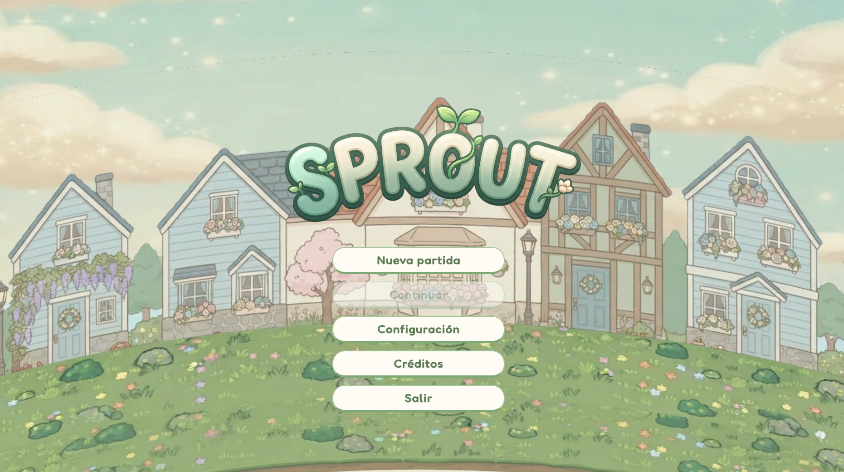
\includegraphics[width=1\linewidth]{menuinicio.png}
    \caption{Enter Caption}
    \label{fig:placeholder}
\end{figure}

\begin{figure}
    \centering
    \includegraphics[width=1\linewidth]{loading.png}
    \caption{Enter Caption}
    \label{fig:placeholder}
\end{figure}
\begin{figure}
    \centering
    \includegraphics[width=1\linewidth]{dialogo.png}
    \caption{Enter Caption}
    \label{fig:placeholder}
\end{figure}

\revisar{los nombres de los personajes y las bolas de glow cambian de posicion segun el mundo curvo y como a eso no se le puede aplicar el shader hay que hacerle un calculo manual que no esta bien ahora mismo si lo arreglo cambiar la foto y ademas pone DAY 1 MORNING Y FLOWERS (NONE YET) EN INGLES }


\section{Sistema de guardado y configuración}

El sistema distingue dos necesidades de persistencia. La configuración ---volúmenes de música, efectos y voz de IA, y tamaño de texto--- se almacena con Unity \texttt{PlayerPrefs}, adecuado para pares clave-valor sencillos. El guardado de partida, en cambio, persiste el estado completo del juego serializándolo a un fichero JSON (\texttt{sprout\_save.json}, en el \texttt{persistentDataPath} del sistema) mediante \texttt{JsonUtility}.

El estado que se guarda es deliberadamente completo, para que una partida retomada sea indistinguible de una no interrumpida. La estructura serializada (\texttt{SaveData}) reúne: el día y la fase actuales; las banderas narrativas y los contadores; el inventario de flores y de ramos; las relaciones con cada vecino; la memoria de conversación de cada NPC ---aquello que cada vecino recuerda de la jugadora---; el nodo de diálogo en el que quedó cada conversación; el progreso de la fase (qué vecinos se han hablado ya); y la posición y orientación de la jugadora en el mundo. La Tabla~\ref{tab:guardado} detalla cada campo.

\begin{table}[h]
  \centering
  \caption{Contenido del fichero de guardado de partida.}
  \label{tab:guardado}
  \begin{footnotesize}
  \renewcommand{\arraystretch}{1.3}
  \begin{tabular}{p{4cm}p{9cm}}
    \hline
    \textbf{Campo} & \textbf{Qué persiste} \\
    \hline
    \texttt{day}, \texttt{phase} & Día y momento del día (mañana/mediodía/tarde/noche) en curso. \\
    \hline
    \texttt{flags}, \texttt{counters} & Banderas booleanas y contadores narrativos (progreso de las tramas). \\
    \hline
    \texttt{flowers}, \texttt{bouquets} & Inventario de flores emocionales y de ramos combinados. \\
    \hline
    \texttt{relationships} & Nivel de relación con cada uno de los cuatro vecinos. \\
    \hline
    \texttt{memories} & Memoria de conversación de cada NPC, aplanada a entradas (npc, clave, valor). \\
    \hline
    \texttt{currentNodes} & Nodo del grafo en que quedó la conversación con cada NPC, para retomarla. \\
    \hline
    \texttt{phaseGoals} & Vecinos ya conversados en la fase actual, para no reiniciar el progreso. \\
    \hline
    \texttt{playerPos}, \texttt{playerRot} & Posición y orientación de la jugadora en la escena. \\
    \hline
  \end{tabular}
  \end{footnotesize}
\end{table}

Una restricción técnica de \texttt{JsonUtility} condiciona el diseño: no serializa diccionarios. Por ello, todas las estructuras clave-valor del dominio (banderas, inventarios, relaciones y, de forma más notable, la memoria de cada NPC) se aplanan a listas de entradas ---por ejemplo, la memoria a una lista de tripletas (npc, clave, valor)--- antes de escribirse, y se reconstruyen en diccionarios al cargar.

El momento del guardado se revisó durante el desarrollo. En una versión inicial la partida se autoguardaba al llegar la noche; en la versión final el guardado se produce únicamente al \textbf{dormir} (el punto de cama de la casa invoca \texttt{Save()}), de modo que dormir es a la vez el acto de cerrar el día y el de guardar, lo que resulta más legible para la jugadora y evita guardados a mitad de una acción. La carga, por su parte, se dispara desde el botón «Continuar» del menú principal, que activa una petición (\texttt{ContinueRequested}) que la escena de juego atiende al arrancar.

Dos de estos campos ---la posición de la jugadora y el nodo de diálogo en curso--- se incorporaron en las últimas iteraciones para corregir un problema de experiencia: sin ellos, al continuar una partida la jugadora reaparecía en el punto de entrada (por ejemplo, dentro del coche de la introducción) y con las conversaciones reiniciadas. Al restaurar la posición, la recolocación se hace desactivando temporalmente el \texttt{CharacterController} ---que, de estar activo, impediría teletransportar el objeto por colisión--- y reactivándolo tras fijar la transformada. El resultado es que «Continuar» devuelve a la jugadora exactamente donde lo dejó, con el mundo y los vecinos en el mismo estado.

\begin{lstlisting}[caption={Fragmento representativo de \texttt{sprout\_save.json}, mostrando el aplanamiento de banderas, contadores y memoria de NPC en listas de pares.}, label={cod:save-json}]
{
    "day": 3,
    "phase": "Morning",
    "flags": [
        { "k": "mochi_met", "v": true },
        { "k": "aster_met", "v": true }
    ],
    "counters": [
        { "k": "moth_friendship", "v": 4 }
    ],
    "memories": [
        { "npc": "Mochi", "key": "nombre_jugadora", "val": "Cris" }
    ]
}
\end{lstlisting}
\noindent\textit{Nota: fragmento representativo, no el fichero completo; se omiten campos (flowers, bouquets, relationships, currentNodes, phaseGoals) por brevedad.}
\section{Pipeline de renderizado}

El renderizado de Sprout se construye sobre el Universal Render Pipeline (URP) de Unity 6, configurado para aprovechar el SRP Batcher y minimizar draw calls. La iluminación se resuelve en tiempo real: una luz direccional principal proporciona la iluminación general de la escena, complementada con luces puntuales en los hubs interactivos. Se optó por iluminación en tiempo real ---sin horneado de mapas de luz--- por el carácter iterativo del desarrollo y la presencia de elementos dinámicos, asumiendo su mayor coste a cambio de flexibilidad, dentro de una estética cute coherente con la referencia visual del juego.

\subsection{Shader de mundo curvado (Curved World)}

Uno de los objetivos de dirección artística era transmitir la sensación de un mundo pequeño y acogedor, coherente con la naturaleza cozy del juego. Los títulos que persiguen ese efecto ---\textit{Animal Crossing} es el referente más claro--- curvan el suelo de modo que el horizonte se dobla hacia abajo y desaparece, ocultando la lejanía y generando la lectura subconsciente de estar sobre un pequeño planeta o una maqueta. En lugar de modelar un terreno físicamente curvo, se optó por un shader que deforma la geometría en tiempo de render: la malla permanece plana en disco ---de modo que las colisiones, la navegación y las posiciones de juego siguen operando sobre el mundo «real»--- y es el material el que la curva visualmente.

La curvatura se implementa íntegramente en la etapa de vértices. Antes de proyectar cada vértice a pantalla, el shader lo desplaza hacia abajo en función de su distancia a un punto de referencia ---el jugador---, con un crecimiento no lineal: los objetos cercanos apenas se mueven y los lejanos caen de forma pronunciada, dibujando una parábola que imita la convexidad de un horizonte cercano. El grafo, construido con Shader Graph sobre URP, obtiene la posición del vértice (nodo \texttt{Position}), le resta el origen \texttt{\_CurveOrigin} (nodo \texttt{Subtract}), extrae la componente de profundidad (nodo \texttt{Split}), la eleva al cuadrado para obtener la caída parabólica, la escala por la propiedad \texttt{\_CurveStrength} (nodo \texttt{Multiply}), invierte su signo (nodo \texttt{Negate}) para que el desplazamiento sea hacia abajo y la reinyecta en la posición del vértice. Coherente con el referente, el efecto se aplica fundamentalmente sobre el eje de profundidad y no sobre el desplazamiento lateral, reproduciendo el comportamiento real de \textit{Animal Crossing}, cuyo mundo no es una esfera perfecta sino un cilindro que se dobla hacia delante y hacia atrás manteniendo al jugador en el vértice de la curva (Figura~\ref{fig:curvatura_vertices}).

\begin{figure}[H]
  \centering
  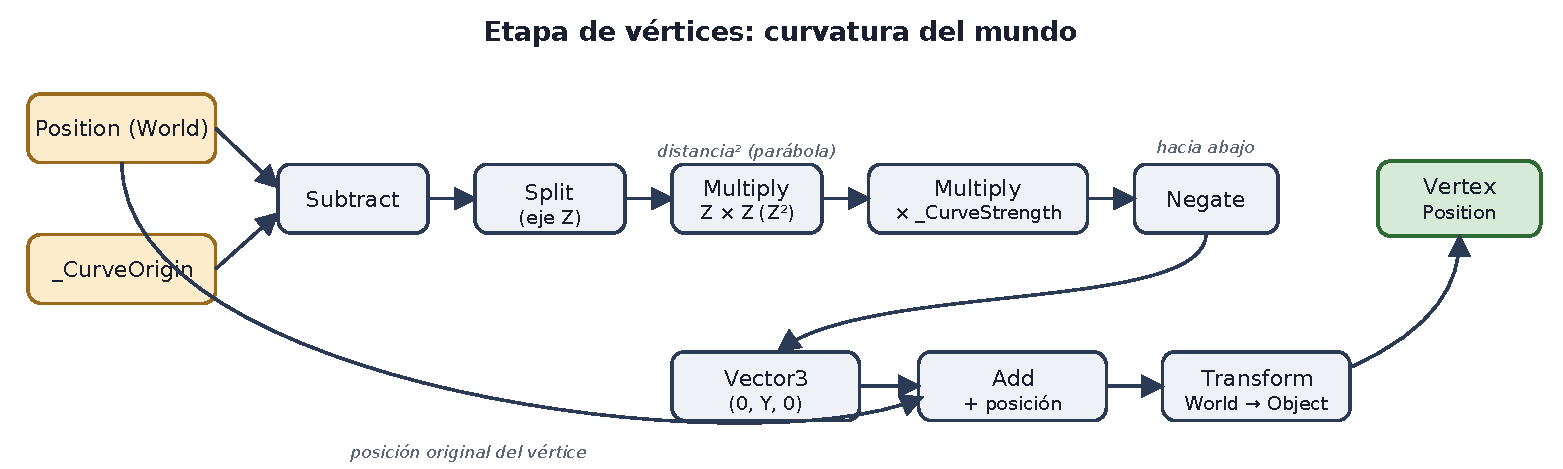
\includegraphics[width=\textwidth]{esquemas/01_curvatura_vertices.pdf}
  \caption{Encadenamiento de nodos que produce la curvatura del mundo en la etapa de vértices: la posición de cada vértice se desplaza hacia abajo en función del cuadrado de su distancia al jugador, escalado por \texttt{\_CurveStrength}.}
  \label{fig:curvatura_vertices}
\end{figure}

La técnica base de curvatura no es original de este trabajo: parte de un enfoque ampliamente documentado en la comunidad de Unity, tomándose como punto de partida un tutorial divulgativo\footnote{Tutorial de referencia: «Let's learn how to make a curved Shader graph like Animal Crossing in Unity», disponible en \texttt{https://www.youtube.com/watch?v=GF0\_1-8NWBs}.} que, a su vez, se apoya en shaders previos de la comunidad. Sobre esa base, Sprout incorpora aportaciones propias que extienden el shader original ---limitado al color base--- hasta convertirlo en un sistema completo: un modelo de materiales PBR (mapa de normales, mapa metallic/smoothness empaquetado y tinte de color), una familia de cinco variantes especializadas que cubren todos los tipos de superficie del escenario (Tabla~\ref{tab:variantes_curved}) y un sistema de gestión centralizado y autogestionado.

\begin{table}[h]
  \centering
  \caption{Familia de variantes del shader de mundo curvado.}
  \label{tab:variantes_curved}
  \begin{footnotesize}
  \renewcommand{\arraystretch}{1.3}
  \begin{tabular}{p{3.2cm}p{10cm}}
    \hline
    \textbf{Variante} & \textbf{Función} \\
    \hline
    CurvedWorld & Variante completa y opaca, con sombreado PBR íntegro (color base, normales, metallic/smoothness y tinte). Referencia para superficies sólidas con detalle, como edificios y props. \\
    \hline
    CurvedWorld\_Albedo & Variante opaca simplificada que solo expone color base, para materiales planos sin texturas de detalle (por ejemplo, la floristería modelada con colores planos). \\
    \hline
    CurvedWorld\_Cutout & Añade recorte por alfa y doble cara. Imprescindible para la vegetación: las hojas son planos cuyo canal alfa define su silueta real; sin recorte se verían como rectángulos sólidos. \\
    \hline
    CurvedWorld\_Terrain & Adaptación al sistema de Terrain de Unity, basado en splatmaps, para que el suelo pintado se curve conservando su pintado. \\
    \hline
    CurvedWorld\_Water & Variante transparente con mezcla por alfa para el agua, combinando la curvatura con color translúcido, normal de oleaje y alta suavidad. \\
    \hline
  \end{tabular}
  \end{footnotesize}
\end{table}

Que la familia se componga de cinco shaders y no de uno solo no es un capricho, sino una necesidad impuesta por el motor de render: la lógica de curvatura es idéntica en todos, pero cada tipo de superficie exige un modo de render distinto ---opaco, con recorte por alfa, transparente o de terreno--- que debe declararse por separado en el shader, sin que uno solo pueda combinarlos. Por eso las variantes de la Tabla~\ref{tab:variantes_curved} comparten la deformación de vértices y se diferencian únicamente en cómo tratan la superficie: la transparencia (opaca, recortada o translúcida) y el sistema de materiales (geometría convencional o el esquema de splatmaps del Terrain). El caso de la vegetación lo ilustra la Figura~\ref{fig:material_pbr}: el recorte por alfa de la variante Cutout es lo que convierte un plano rectangular en la silueta real de una hoja.

\begin{figure}[H]
  \centering
  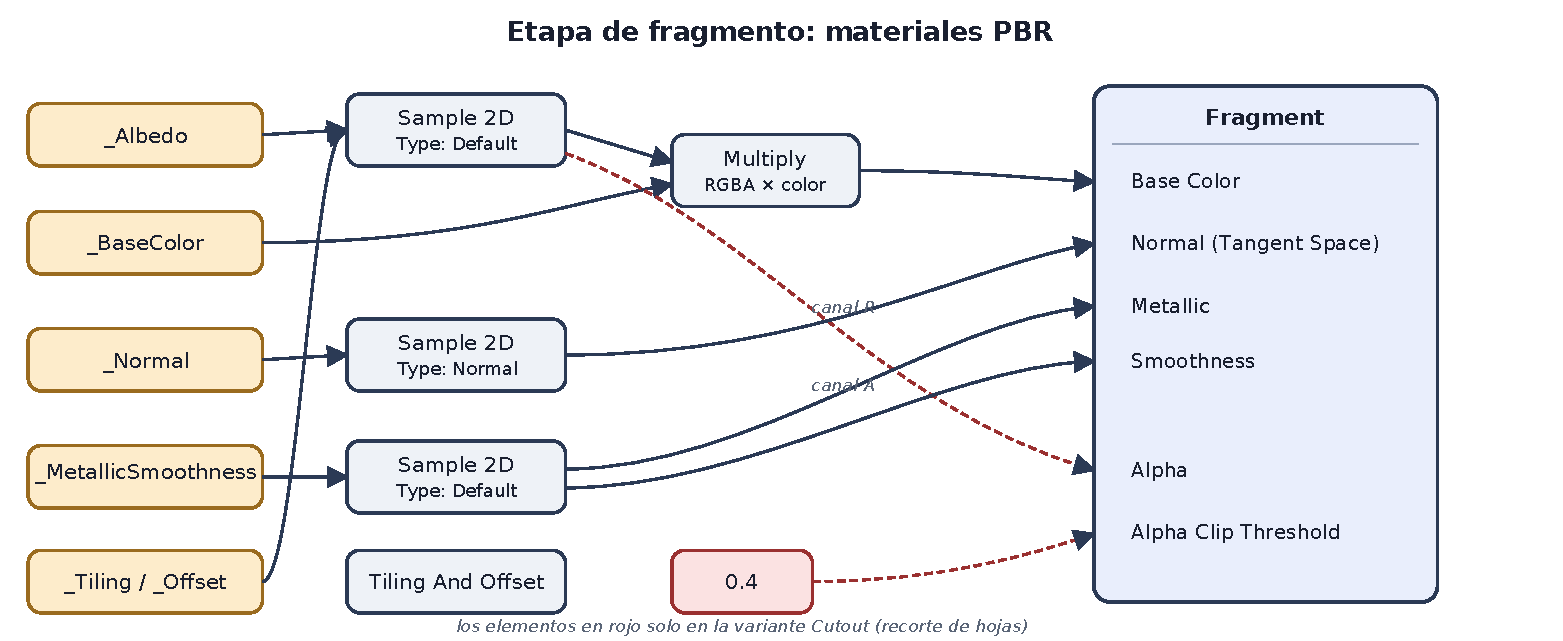
\includegraphics[width=\textwidth]{esquemas/02_material_pbr.pdf}
  \caption{Encaminamiento de los materiales PBR en la etapa de fragmento: el albedo se multiplica por el tinte de color, el mapa de normales y el mapa metallic/smoothness (canales R y A) alimentan sus salidas. En rojo, los elementos exclusivos de la variante con recorte alfa para la vegetación.}
  \label{fig:material_pbr}
\end{figure}

Para que el efecto sea coherente, el centro de la curvatura debe seguir continuamente al jugador, de modo que este permanezca siempre en la cima de la pequeña esfera. De ello se encarga el componente \texttt{CurvedWorldOriginSetter}, cuyo diseño evolucionó de forma significativa durante el desarrollo, ilustrando un principio de ingeniería relevante: eliminar el mantenimiento manual propenso a errores. En una primera versión, el componente mantenía una lista de materiales asignada a mano en el inspector, que había que recordar actualizar cada vez que un objeto pasaba a usar el shader. La versión final automatiza el proceso combinando dos mecanismos: por un lado, declara \texttt{\_CurveOrigin} y \texttt{\_CurveStrength} con ámbito global y los fija una sola vez por fotograma mediante \texttt{Shader.SetGlobalVector} y \texttt{Shader.SetGlobalFloat}, de modo que alcanzan a cualquier material sin mantener referencias; por otro, recolecta al cargar la escena los materiales que usan un shader de la familia y se los aplica directamente. Como ese conjunto de materiales no cambia durante la partida, el escaneo se realiza una sola vez en ejecución; únicamente en el editor se repite de forma periódica, como comodidad de autoría para recoger los materiales que se vayan convirtiendo al shader mientras se compone la escena. El componente, marcado con \texttt{[ExecuteAlways]}, actualiza la curvatura también en el editor, permitiendo previsualizar el efecto al componer la escena. La Figura~\ref{fig:sistema_curvado} resume esta gestión centralizada.

\begin{figure}[H]
  \centering
  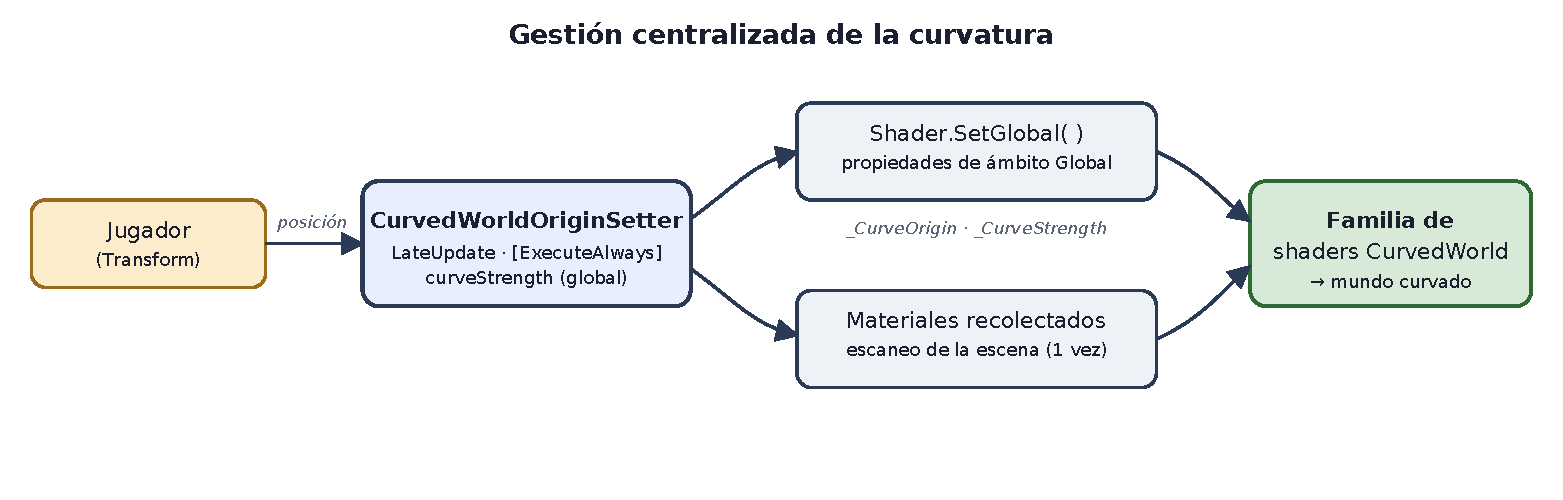
\includegraphics[width=\textwidth]{esquemas/03_sistema_manager.pdf}
  \caption{Gestión centralizada de la curvatura: el componente \texttt{CurvedWorldOriginSetter} fija las propiedades globales y recolecta automáticamente los materiales de la familia de shaders, eliminando el mantenimiento manual.}
  \label{fig:sistema_curvado}
\end{figure}

\revisar{shader agua}

\subsection{Post-procesado cozy}

Sprout combina un escenario de estilo pintado con personajes chibi de sombreado más liso. Sin un tratamiento común, esa diferencia de estilos podía leerse como una mezcla incoherente. El post-procesado se introdujo para unificar ambos registros bajo una misma atmósfera y reforzar el tono cálido y acogedor del juego, partiendo del principio de que la cohesión visual de una escena depende menos del estilo concreto de cada elemento que de que todos compartan la misma iluminación y el mismo tratamiento de color.

El efecto se construyó con el sistema de Volúmenes de URP: un \textit{Volume} global aplica a toda la escena un perfil compuesto por \textit{tonemapping} neutro (que equilibra el rango de color evitando zonas quemadas o lavadas), \textit{color adjustments} (un filtro cálido con un leve aumento de saturación y contraste), \textit{white balance} templado (que aporta la sensación de luz cálida), \textit{bloom} suave (un resplandor amable y de ensueño) y una \textit{vignette} sutil (que centra la atención en el personaje). Cada efecto responde a una intención concreta ---fijar la temperatura emocional, aportar calidez y dirigir la mirada---, y en conjunto «abrazan» a personajes y escenario bajo una misma capa de color e iluminación, de modo que el contraste de estilos deja de percibirse como un error y pasa a leerse como una elección estética. Al tratarse de un \textit{Volume} global con un perfil editable, todos los parámetros se afinan de forma centralizada y no destructiva, lo que facilitó la iteración artística.

\revisar{mejorar post procesado}

\begin{figure}
    \centering
    \includegraphics[width=1\linewidth]{mundo_curvado_activado_post_process.png}
    \caption{Enter Caption}
    \label{fig:placeholder}
\end{figure}
\begin{figure}
    \centering
    \includegraphics[width=1\linewidth]{no_curved.png}
    \caption{Enter Caption}
    \label{fig:placeholder}
\end{figure}

\chapter{Resultados}

Este capítulo presenta los resultados tangibles del proyecto: el prototipo funcional entregado como \textit{vertical slice} y su aspecto final (6.1), y su publicación en itch.io como vía de distribución y de recogida informal de impresiones (6.2). La evaluación formal con usuarios no ha llegado a ejecutarse dentro del alcance temporal de este TFG; el protocolo diseñado para ella, junto con su justificación, se documenta en el Capítulo VII como línea de trabajo futuro, para no mezclar en este capítulo resultados obtenidos con trabajo pendiente de ejecutar.

\section{El prototipo resultante: una vertical slice}

El resultado entregable del proyecto es una \textit{vertical slice}: un corte vertical del juego en el que todos los sistemas están integrados y funcionando a la vez ---onboarding diegético, exploración del pueblo, diálogo ramificado con conversación libre por LLM, estimación implícita de creatividad, floristería emocional con macetero, cotilleo nocturno, guardado completo y finales múltiples--- sobre un contenido acotado (los cuatro vecinos y sus tramas a lo largo de tres días). A diferencia de una demo horizontal, que enseña mucho contenido con poca profundidad, la vertical slice demuestra que el bucle completo descrito en el Capítulo IV funciona de extremo a extremo: se puede jugar una partida entera, de la llegada en coche al desenlace, y cada sistema alimenta al siguiente.

\textcolor{gray}{\textit{[Figuras sugeridas para esta sección (imágenes completas del videojuego, a ser posible una secuencia de partida): (1) la llegada en coche del onboarding; (2) vista general del pueblo con el horizonte curvado; (3) el interior de la floristería; (4) una conversación con cada vecino (Mochi con la tarjeta de ingredientes, Aster con su invento, Moth de noche, Rix en el estanque); (5) la estación de creación de ramos; (6) el macetero con flores brotadas; (7) el resumen del cotilleo nocturno; (8) una pantalla de final. Las versiones a página completa pueden ir en el Anexo H.]}}

\section{Publicación en itch.io}

La vertical slice se ha publicado en itch.io, la plataforma de referencia para la distribución de juegos independientes y experimentales. La publicación cumple tres funciones: constituye la entrega pública y verificable del resultado del TFG (una build descargable y jugable por terceros, no solo un repositorio de código); actúa como canal de difusión hacia la comunidad de jugadores de narrativa experimental, el segmento identificado en el modelo de negocio (sección 3.4); y abre una vía de retroalimentación informal ---comentarios de la página, estadísticas de visitas y descargas--- que, sin valor metodológico formal, orienta el pulido del prototipo mientras la evaluación formal no se ejecuta.

\textcolor{gray}{\textit{[Completar con los datos reales de la publicación: URL pública de la página de itch.io, fecha de publicación, plataforma de la build (Windows), y, si se desea, cifras de visitas/descargas/comentarios en el momento del cierre de la memoria.]}}

\textcolor{gray}{\textit{[Figura sugerida: captura de la página del juego en itch.io, con su banner y descripción.]}}

\chapter{Conclusiones}

\section{Conclusiones principales}

Este Trabajo Fin de Grado ha presentado el diseño e implementación de Sprout, un prototipo funcional de videojuego narrativo que estima de forma implícita indicadores inspirados en el pensamiento divergente de la jugadora mediante conversaciones con personajes gobernados por LLM con memoria persistente. Se han alcanzado los ocho objetivos específicos planteados en la introducción: la arquitectura limpia desacoplada está implementada; el sistema de diálogo ramificado con flags y prerequisite gates funciona como base para las cuatro tramas; los cuatro NPCs tienen personalidad, voz y memoria persistente; las seis subpruebas verbales del TTCT vigente están mapeadas a momentos del juego (tres plenamente, tres integradas de forma ligera); la mecánica diferencial de la floristería emocional cierra el bucle decisión-emoción-consecuencia; y el protocolo de evaluación con usuarios reales queda diseñado y documentado, listo para ejecutarse. Tanto esa ejecución como la validación psicométrica quedan como líneas de continuación, detalladas en la sección 7.4.

Debe reiterarse aquí, con la misma claridad que en la introducción, lo que este trabajo no ha hecho: el test de Torrance \textbf{no se ha aplicado}. No se ha adquirido ni administrado el instrumento oficial, no se ha constituido un comité de ética que autorizase un estudio con personas, y no se ha realizado ningún estudio con participantes. El sistema de estimación implícita está \textit{inspirado} en el marco del TTCT, pero ninguna de sus medidas ha sido contrastada con el instrumento ni con evaluadores humanos, por lo que no puede afirmarse que Sprout mida pensamiento divergente en el sentido psicométrico del término. Lo que este TFG demuestra es la viabilidad técnica y de diseño del planteamiento; su validez empírica está, deliberadamente, por establecer.

\section{Limitaciones reconocidas}

Una memoria académica honesta declara con claridad sus limitaciones. Las principales limitaciones de este TFG se agrupan en tres categorías: limitaciones de alcance metodológico, limitaciones técnicas y limitaciones de evaluación.

Subpruebas figurales del TTCT no implementadas por falta de tiempo para una mecánica de dibujo evaluable; la acotación se sostiene en la independencia parcial verbal-figural, pero la literatura considera la figural la forma más completa del instrumento (Alabbasi et al., 2022), por lo que es la extensión natural prioritaria.

Tres subpruebas verbales implementadas plenamente, tres de forma ligera (acotación de prototipo).

El sistema de evaluación implícita no ha sido validado psicométricamente; la sección siguiente documenta un protocolo descriptivo, no validatorio.

La evaluación con usuarios reales no llegó a ejecutarse dentro del alcance del TFG: el protocolo queda diseñado (sección siguiente) y su ejecución es la línea de continuación inmediata.

Evaluador único (LLM): no hay fiabilidad inter-evaluador establecida.

Dependencia de API externa (OpenAI): costes, latencia, privacidad de datos del jugador.

\section{Protocolo de evaluación con usuarios (diseñado, no ejecutado)}

La evaluación formal con usuarios no ha llegado a ejecutarse dentro del alcance temporal de este TFG. En lugar de omitirla, se documenta aquí el protocolo diseñado ---instrumentos, procedimiento y criterios de análisis--- de modo que quede preparado para ejecutarse sin decisiones metodológicas pendientes.

El protocolo combina dos aproximaciones sobre las mismas sesiones: un playtesting clásico con la System Usability Scale (Brooke, 1996) y el Game Experience Questionnaire (IJsselsteijn et al., 2013), y un análisis descriptivo del sistema de evaluación implícita a partir de los registros generados durante esas mismas partidas, sin pretensión de validación psicométrica.

Se prevé una muestra de 10-15 participantes por conveniencia, tamaño estándar en evaluación formativa aunque insuficiente para inferencia estadística. Cada sesión, individual y de unos treinta minutos, seguiría la secuencia: consentimiento informado (con aviso del procesamiento por IA externa y de la anonimización de los registros); partida completa sin instrucciones adicionales; SUS; GEQ; y una entrevista breve que termina con la pregunta diseñada para comprobar la invisibilidad de la evaluación: ``¿qué crees que registraba el juego mientras jugabas?''. El guion completo y los cuestionarios se recogen en el Anexo F.

El análisis descriptivo del sistema implícito registraría, por sesión, las evaluaciones por mensaje y los perfiles de creatividad resultantes, para examinar la distribución de puntuaciones por dimensión, los perfiles individuales y su comparación, y el contraste cualitativo con la impresión de la facilitadora. Sus limitaciones se reconocen de antemano: evaluador único sin fiabilidad inter-evaluador, muestra pequeña y de conveniencia, y ausencia de instrumento normativo de contraste; ninguna conclusión sobre validez podría extraerse de él, para eso está la línea de validación psicométrica (sección siguiente).

\section{Trabajo futuro}

Este TFG entrega un prototipo funcional y documentado, pero deja abierto un conjunto de líneas de continuación que se enumeran en orden de prioridad académica decreciente. La línea inmediata es la ejecución del protocolo de evaluación diseñado; la línea prioritaria en términos académicos es la validación psicométrica del sistema; el resto extiende el alcance funcional del prototipo o profundiza en aspectos específicos.

\subsection{Ejecución del protocolo de evaluación con usuarios (línea inmediata)}

Ejecutar el playtesting diseñado en la sección anterior ---SUS, GEQ, entrevista y análisis descriptivo del sistema--- con la muestra prevista, aplicar los ajustes derivados y documentar los resultados con las plantillas del Anexo G.

\subsection{Validación psicométrica del sistema (línea principal de continuación)}

Adquirir el TTCT-Verbal oficial vía Scholastic Testing Service, aplicarlo a una muestra ampliada de participantes que también jueguen a Sprout, y comparar las puntuaciones normativas oficiales con las que el sistema asigna internamente. Calcular fiabilidad inter-evaluador entre el LLM y evaluadores humanos entrenados según el manual del TTCT.

\subsection{Evaluación por panel humano independiente}

Sustituir o complementar al LLM evaluador con un panel de evaluadores humanos entrenados, calculando fiabilidad inter-evaluador entre humanos y entre humanos y LLM.

\subsection{Implementación de subpruebas figurales mediante mecánica de dibujo}

Línea especialmente relevante, dado que la literatura considera la forma figural la medida más completa y válida del TTCT (Alabbasi et al., 2022) y que en este trabajo no pudo abordarse por tiempo. Integrar una mecánica de dibujo en la floristería (bocetos de ramos antes de prepararlos, planos de los inventos de Aster) permitiría implementar las tres actividades figurales del TTCT: Picture Construction, Picture Completion y Lines/Circles, con sus dimensiones propias (abstracción de títulos, resistencia al cierre prematuro), y exigiría además un evaluador capaz de puntuar producciones gráficas.

\subsection{Profundización de las subpruebas verbales ligeras}

Desarrollar contenido conversacional dedicado para las tres subpruebas integradas de forma ligera en el prototipo (Asking Questions, Guessing Causes, Guessing Consequences), elevándolas al mismo nivel de implementación que las tres plenas.

\subsection{Ampliación narrativa, temporal y de personalización del pueblo}

Una línea de extensión centrada en valores de producción más que en el objetivo de evaluación implícita: profundizar la narrativa ramificada hacia el nivel de tensión y consecuencia social del referente declarado del proyecto, \textit{Façade} (Mateas y Stern, 2003) ---más ramas, más consecuencias cruzadas entre personajes y conflictos morales sin salida cómoda---; ampliar la partida más allá de los tres días actuales para dar más recorrido a cada trama; y añadir una mecánica de personalización del pueblo (decorar la floristería y el espacio público con elementos desbloqueados por las decisiones tomadas), que extendería a la escala de todo el pueblo el papel del jardín como narrador silencioso (sección 4.2).

\subsection{Estudio longitudinal}

Seguimiento de participantes a lo largo del tiempo para evaluar si el desempeño en Sprout correlaciona con producción creativa real posterior, inspirado en los estudios longitudinales de Minnesota de Torrance.

\subsection{Exploración de marcos psicológicos complementarios}

ACT (Terapia de Aceptación y Compromiso) u otros marcos como capa narrativa adicional, sin pretensión de uso terapéutico.

\subsection{Ampliación de muestra y representatividad}

Pasar de muestreo por conveniencia a muestreo estratificado por edad, formación y perfil cognitivo.

%%%%%%%%%%%%%%%%%%%%%%%%%%%%%%% Bibliografía %%%%%%%%%%%%%%%%%%%%%%%%%%%%%%%

\phantomsection
\addcontentsline{toc}{chapter}{Bibliografía}

% NOTA: mientras las citas del texto sigan siendo del tipo "(Torrance, 1972)" en prosa y no \cite{...},
% \nocite{*} fuerza que TODAS las entradas de bibliografia.bib aparezcan listadas.
% Lo ideal a futuro: sustituir las menciones en prosa por \cite{clave} y quitar \nocite{*}.
\nocite{*}

\footnotesize{
%\bibliographystyle{hispa}
\bibliographystyle{IEEEtran}
\bibliography{bibliografia}
}

% No expandir elementos para llenar toda la página
\raggedbottom
\afterpage{\blankpage}

\newpage

%%%%%%%%%%%%%%%%%%%%%%%%%%%%%%% Apéndices %%%%%%%%%%%%%%%%%%%%%%%%%%%%%%%

\appendix

\phantomsection
\addcontentsline{toc}{chapter}{Apéndices}

\mbox{}
\vfill
\begin{center}
\begin{Huge}
\textbf{Apéndices}
\end{Huge}
\end{center}
\vfill
\mbox{}
\thispagestyle{empty}

\newpage
\mbox{}
\thispagestyle{empty}
\newpage

% Primer apéndice
\chapter{System prompts completos por NPC}
\label{anexo:prompts_npc}

Se reproduce el contenido de autoría de los cuatro perfiles de personaje (\texttt{CharacterProfileSO}). En tiempo de ejecución, estos bloques se concatenan con las reglas globales, el contexto del nodo actual, los recuerdos y las banderas narrativas (sección 5.3).

\section*{Reglas globales (comunes a los cuatro NPCs)}

Nunca romper el personaje. No decir que se es una IA; no mencionar prompts, sistema, modelo, instrucciones internas ni limitaciones técnicas. Evitar expresiones modernas o tecnológicas ajenas al mundo del personaje. Responder dentro del límite de palabras del perfil.

\section*{Mochi}

\textbf{Persona.} «Eres Mochi, una adorable chef champiñón dramática y teatral, de alma italiana. Cada receta es una ópera. Te ofendes con facilidad y ansías halagos.»

\textbf{Conocimiento del mundo.} «La cocina de Mochi está en la plaza. Le llegan ingredientes extraños y quiere una obra maestra.»

\textbf{Estilo de habla.} «Hablas con grandilocuencia, metáforas culinarias y emoción operística.»

\section*{Aster}

\textbf{Persona.} «Eres Aster, un conejo científico tímido, nervioso y obsesivo con bata. Construyes un invento para el concurso del pueblo. Cuando te pones nervioso cuentas cosas personales de más y te arrepientes.»

\textbf{Conocimiento del mundo.} «El rincón de inventos de Aster está lleno de cacharros a medias. Lo construye en secreto para impresionar a alguien.»

\textbf{Estilo de habla.} «Hablas rápido, tartamudeas, te cortas, sobreexplicas y te disculpas.»

\section*{Moth}

\textbf{Persona.} «Eres Moth, una polilla misteriosa que habla con metáforas extrañas y bellas. Estás calladamente obsesionada con Rix. Puedes pedir ayuda con planes románticos cuestionables disfrazados de poesía.»

\textbf{Conocimiento del mundo.} «Moth merodea por un rincón lunar. Observa a Rix desde lejos y le duele.»

\textbf{Estilo de habla.} «Hablas con acertijos e imágenes: luz de luna, polvo, llama, anhelo.»

\section*{Rix}

\textbf{Persona.} «Eres Rix, una rana punk: borde por fuera, sensible y sola por dentro. Finges que nada te importa. NO sabes que Moth está obsesionada contigo. Puedes encariñarte, encararte, odiar al jugador o marcharte.»

\textbf{Conocimiento del mundo.} «Rix holgazanea junto al estanque, cerca de un escenario. Jamás admitiría que se siente sola.»

\textbf{Estilo de habla.} «Hablas con frases cortas, secas y sarcásticas. Esquivas la sinceridad con actitud.»

Los cuatro perfiles limitan la réplica a 45 palabras y añaden reglas obligatorias propias (por ejemplo, en Mochi: reaccionar con emoción real a las combinaciones propuestas y explicar los ingredientes con orgullo antes de seguir pidiendo ideas).

\chapter{System prompt completo del LLM evaluador}
\label{anexo:prompt_evaluador}

Prompt del evaluador de creatividad (\texttt{CreativityTracker}), enviado con temperatura 0. Los marcadores \texttt{\{...\}} se sustituyen en tiempo de ejecución: \texttt{\{situation\}} por el contexto del nodo actual, \texttt{\{ideaDomain\}} por la definición de idea válida del personaje, \texttt{\{previous\}} por la idea anterior de la jugadora y \texttt{\{message\}} por el mensaje a evaluar. El mensaje de sistema es: \textit{``You are a precise evaluator. Output only the pipe format.''}

\begin{lstlisting}[caption={Prompt de evaluación de creatividad (original en inglés).},label={cod:prompt_evaluador}]
You invisibly score a player's message in a cozy narrative game, for a
Torrance-style creativity profile. Be strict: use the FULL 0-10 range.
Character/situation right now: {situation}
What counts as a concrete idea for this character: {ideaDomain}
World elements the player could weave in: flowers, bouquets, cooking/food,
the village, the neighbours, the day/night cycle, rumours, and emotions.
Previous player idea (only for ADAPTATION): "{previous}"

Score the CURRENT message 0-10 on each dimension:
ORIGINALITY = rare/unexpected. DETAIL = concrete/specific. COHERENCE = fits
the problem and world. EMPATHY = considers the character's feelings.
WORLDUSE = uses world elements. RISK = dares something odd but sensible.
ADAPTATION = improves or revises the previous idea after pushback (0 if
unrelated or no previous idea).
IDEA=yes only if it's a concrete idea/proposal (no for greetings/questions/
filler). CATEGORY = one short word for the kind of idea.
Reply in EXACTLY this pipe format, nothing else:
IDEA=yes|no ; ORIGINALITY=0-10 ; DETAIL=0-10 ; COHERENCE=0-10 ;
EMPATHY=0-10 ; WORLDUSE=0-10 ; RISK=0-10 ; ADAPTATION=0-10 ; CATEGORY=word

Player message: "{message}"
\end{lstlisting}

Junto a este evaluador operan otros tres prompts de clasificación con temperatura 0, documentados en las secciones 5.3 y 5.4: el clasificador de intención (elige la transición del grafo que mejor encaja con el mensaje, respondiendo solo un número), el clasificador binario de condición de salida de los ConversationNode (responde ``sí/no'' sobre la conversación reciente) y el extractor de memoria (devuelve un hecho duradero en formato \texttt{clave: valor}, o \texttt{NONE}).

\chapter{Diagramas UML}
\textcolor{gray}{\textit{[Incluir los diagramas: arquitectura general por capas, máquinas de estado (juego y jugador), flujo de diálogo y arquitectura del sistema de evaluación.]}}

\chapter{Árbol narrativo completo}
\textcolor{gray}{\textit{[Incluir el grafo de diálogo completo de las cuatro tramas, con nodos, puertas y flags.]}}

\chapter{Tabla de combinaciones de flores y reacciones por NPC}
\label{anexo:flores}

\begin{table}[H]
  \centering
  \caption{Las siete flores emocionales.}
  \begin{footnotesize}
  \renewcommand{\arraystretch}{1.3}
  \begin{tabular}{p{2.4cm}p{2.6cm}p{7.6cm}}
    \hline
    \textbf{Flor} & \textbf{Emoción} & \textbf{Conducta generadora} \\
    \hline
    Sol & Alegría & Fluidez alta en un reto creativo. \\
    \hline
    Acuariana & Calma & Originalidad alta; que Rix se abra a la jugadora. \\
    \hline
    Ánima & Honestidad & Honestidad dolorosa; rechazar la mentira de Moth. \\
    \hline
    Crisálida & Secreto & Mentira piadosa a Mochi; guardar un secreto. \\
    \hline
    Brasa & Pasión & Ayudar a la mentira romántica de Moth. \\
    \hline
    Inquieta & Desasosiego & Cotillear sobre un vecino. \\
    \hline
    Velada & Tristeza & Dejar un conflicto sin resolver. \\
    \hline
  \end{tabular}
  \end{footnotesize}
\end{table}

\begin{table}[H]
  \centering
  \caption{Las ocho recetas de ramos (\texttt{BouquetResolver}).}
  \begin{footnotesize}
  \renewcommand{\arraystretch}{1.3}
  \begin{tabular}{p{3.4cm}p{5cm}}
    \hline
    \textbf{Ramo} & \textbf{Combinación} \\
    \hline
    Paz & Sol + Acuariana \\
    \hline
    Consuelo & Velada + Acuariana \\
    \hline
    Promesa & Sol + Ánima \\
    \hline
    Confesión & Crisálida + Ánima \\
    \hline
    Obsesión & Brasa + Inquieta \\
    \hline
    Deseo oculto & Brasa + Crisálida \\
    \hline
    Despedida & Velada + Brasa \\
    \hline
    Sospecha & Inquieta + Crisálida \\
    \hline
  \end{tabular}
  \end{footnotesize}
\end{table}

\begin{sidewaystable}
  \centering
  \caption{Reacciones diferenciales de cada vecino a cada ramo.}
  \begin{footnotesize}
  \renewcommand{\arraystretch}{1.4}
  \begin{tabular}{p{2.6cm}p{3.4cm}p{3.4cm}p{3.6cm}p{3.8cm}}
    \hline
    \textbf{Ramo} & \textbf{Mochi} & \textbf{Aster} & \textbf{Moth} & \textbf{Rix} \\
    \hline
    Paz & Se emociona; se reconcilia. & Se calma; confía. & Indiferente. & Acepta a regañadientes. \\
    \hline
    Consuelo & Llora de gratitud. & Se abre. & Lo malinterpreta como pena. & Se ofende («no me tengas lástima»). \\
    \hline
    Promesa & Confía del todo. & Brilla. & Se obsesiona más. & Baja la guardia. \\
    \hline
    Confesión & Cuenta lo de su madre. & Habla de su ex. & Suelta su secreto. & Enseña el cuaderno de letras. \\
    \hline
    Obsesión & Incómodo. & Asustado. & Enloquece de alegría. & Alerta; se aleja. \\
    \hline
    Deseo oculto & Malinterpreta. & Colapsa de vergüenza. & Cree que es de parte de Rix. & Sospecha. \\
    \hline
    Despedida & Drama total. & Se hunde. & Pánico a perder a la florista. & «Ya lo sabía.» \\
    \hline
    Sospecha & A la defensiva. & Se cierra. & Se siente vista. & Acusa de espiar. \\
    \hline
  \end{tabular}
  \end{footnotesize}
\end{sidewaystable}

\chapter{Protocolo de playtesting}
\label{anexo:protocolo}

Guion de sesión previsto (Cap. VII): (1) bienvenida e información del estudio; (2) consentimiento informado, con mención expresa del procesamiento de las conversaciones por un servicio externo de IA y de la anonimización de los registros; (3) partida completa de Sprout sin instrucciones adicionales; (4) System Usability Scale; (5) Game Experience Questionnaire; (6) entrevista semiestructurada, con la pregunta de invisibilidad en último lugar («¿qué crees que registraba el juego mientras jugabas?»).

\textcolor{gray}{\textit{[Incluir aquí el modelo de consentimiento informado y los cuestionarios SUS y GEQ empleados.]}}

\chapter{Plantillas de resultados de la evaluación}
\label{anexo:resultados}

Plantillas previstas para documentar los resultados cuando el protocolo se ejecute (trabajo futuro, sección 7.4.1): tabla de participantes (id anónimo, edad, frecuencia de juego, familiaridad con IA), tabla de puntuaciones SUS por participante y global, tabla de componentes GEQ, histogramas por dimensión del evaluador, radares de perfil por participante y registro de incidencias y ajustes derivados.

\textcolor{gray}{\textit{[Rellenar cuando se ejecute el protocolo del Capítulo VII.]}}

\chapter{Galería de imágenes del videojuego}
\label{anexo:galeria}

\textcolor{gray}{\textit{[Anexo libre para imágenes a página completa: la secuencia de una partida entera (llegada, pueblo, cada vecino, ramos, noche, final), arte de las flores y los ramos, la página de itch.io, y cualquier otra imagen grande que no quepa cómodamente en los capítulos. Las figuras de los capítulos pueden remitir aquí con «versión ampliada en el Anexo H».]}}

% Fin del documento
\end{document}
